\section{Track and primary vertex reconstruction}
The CMS tracker gets traversed by $\mathcal{O}(1000)$ charged particles at each bunch crossing, produced by several proton-proton interactions happening ~simultaneously. This makes track reconstructions extremely challenging, and is the reason why a high granularity of the tracker is vital.
The average number or vertices per event for the whole Run 2 data taking period is shown in Figure~\ref{fig:objreco:pu}, with an average of 34 interactions per bunch crossing.
\begin{figure}[h] 
    \centering
    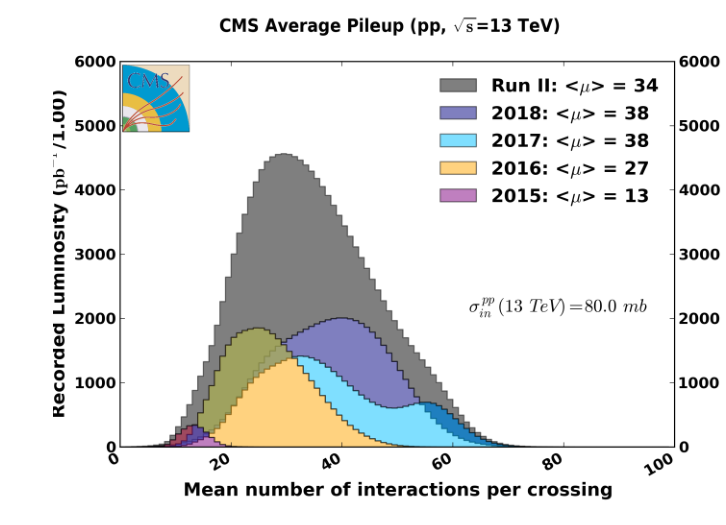
\includegraphics[width=0.49\textwidth]{figures/event_reconstruction/pu.pdf}
    \caption{The average number of vertices per event in CMS for the whole Run 2 data taking period~\cite{CMSlumi}.}
    \label{fig:objreco:pu}
\end{figure}
Track reconstruction encompasses the process of taking hits from the pixel and strip detectors, combining them into particle trajectories, and then estimating the momentum and flight direction of the charged particle responsible for producing the hits. It is a computationally heavy process and at CMS it is based on what is called a combinatorial Kalman filter~\cite{BILLOIR1989390}. A Kalman filter is an algorithm that uses time-dependent observations in order to estimate unknown variables, by proceeding progressively from one measurement to the next, improving the knowledge of the
trajectory with each new measurement. The track reconstruction software in CMS (called the Combinatorial Track Finder (CTF)) constructs its collection of tracks by iteratively looping over the hits and reconstructing tracks, then removing those hits which are already used as inputs for a previous track. It starts from a seed in the innermost tracker layers, usually two or three hits, and then extrapolates the seed trajectories searching for additional hits to associate to that candidate. It then disregards tracks that fail certain criteria  based on a $\chi^2$ calculation, taking both hit and trajectory uncertainties into account, as well as the number of missing hits.
The track reconstruction algorithm is effective over the full range of the tracker coverage, up to $|\eta|<2.5$, and can reconstruct particles with momenta as low as 0.1 GeV and particles which are produced up to 60 \cm from the beam line. In the central region, particles with a momentum of 100 GeV have a \PT-resolution of roughly 2.8 \%, a transverse impact parameter resolution of 10 $\micron$ and a longitudinal impact parameter of 30 $\micron$. 

In order to define the location and uncertainty of every proton-proton interaction in an event, primary-vertex reconstruction is performed. Primary vertices lie within a radius of a few millimeters from the beam axis and are defined as the common origin of groups of tracks.
The reconstruction algorithm takes as input the reconstructed tracks from the previous step which pass certain selection criteria, clusters the tracks that share a common origin, and then fit for the position of each vertex. Each track must have at least 2 hits in the pixel layers and no less than 5 hits in the pixel plus strip layers, as well as a $\chi^2<20$ from a fit to the particle trajectory, to be considered as input for the vertex finder. The primary vertex resolution is around 12 \micron in x and 10 \micron in z for vertices with at least 50 tracks.

Offline, all events are required to have at least one primary vertex reconstructed within a 24 \cm window along the beam axis, with a transverse distance from the nominal interaction region of less than 2 \cm. The reconstructed vertex with the largest value of $\PT^2$ of the summed particles is selected as the primary interaction vertex where the hard scattering process occurred.

\section{The Particle Flow Algorithm}

After track reconstruction, what remains is an incoherent collection of tracks, calorimeter clusters and hits in the muon chambers. In order to connect these, CMS uses an algorithm called Particle Flow (PF)~\cite{1748-0221-12-10-P10003} to combine the information obtained from all sub-detectors in order to infer which particles were actually produced in the event.
The reconstructed physics objects in the order of which they are reconstructed are
\begin{itemize}
  \itemsep0em 
  \item muons, through hits in the tracker and in the muon chambers;
  \item charged hadrons, through hits in the tracker and energy deposits in the calorimeters;
  \item neutral hadrons, through energy deposits in the calorimeters but no hits in the tracker;
  \item photons, through energy deposits in the ECAL but not in the HCAL, and no hits in the tracker; and
  \item electrons, through hits in the tracker and energy deposits in the ECAL.
\end{itemize}

How these different particles propagate through the CMS detector is illustrated in Figure~\ref{fig:objreco:PF}.
\begin{figure}[h!] 
    \centering
    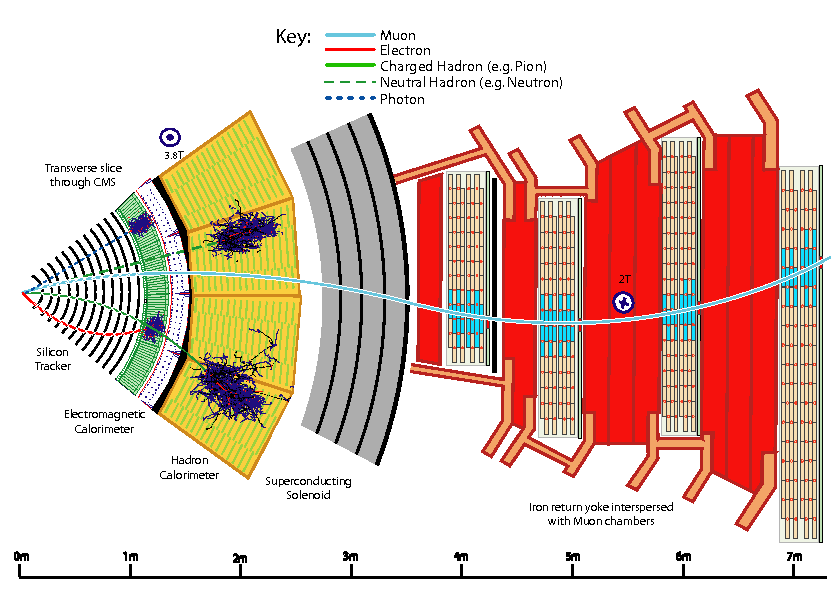
\includegraphics[width=0.79\textwidth]{figures/event_reconstruction/PF.png}
    \caption{Particle interactions in the different subdetectors for a transverse slice through the CMS detector~\cite{1748-0221-12-10-P10003}.}
    \label{fig:objreco:PF}
\end{figure} 

\subsection{Reconstruction of the Particle Flow inputs}

\subsubsection{Electron tracking}
\label{subsub:objreco:electrontracking}
Electron seeding is done in two different ways: ECAL-based  or tracker-based. In the ECAL-based method, electrons are seeded from  ECAL clusters with $E_T > 4 \GeV$, where the position of the cluster is used to infer which hits in the inner tracker belongs to a given electron or positron. As a large fraction of the electron/positron energy is emitted through bremsstrahlung before even reaching the ECAL, the ECAL superclusters covering a small window in $\eta$ and a larger window in $\phi$ are defined in order to fully contain the electron as well as its bremsstrahlung photons. As these superclusters are prone to contamination, tight isolation requirements need to be applied, leading to reconstruction inefficiencies. Therefore, an additional tracker-based seeding approach has been developed. All tracks with $\PT>2\GeV$ are used as potential electron seeds. These tracks are then extrapolated to the ECAL and matched to the closest ECAL cluster. The ratio of the cluster energy to the track momentum is required to be $\sim 1$. The electron candidates are then fit with a Gaussian-sum filter (GSF)~\cite{0954-3899-31-9-N01} and required to pass certain criteria based on the score of a boosted-decision-tree (BDT), which combines the number of tracker hits, the $\chi^2$ of the GSF track, the energy loss along the  track, and the distance between the extrapolated track to the closest ECAL cluster.

\subsubsection{Muon tracking}
\label{subsub:objreco:muontracking}
Muon tracking consists of two parts: the muon spectrometer allows muons to be identified with high efficiency over the full pseudorapidity range, while maintaining a low background due to the absorbing calorimeter layers upstream. The inner tracker on the other hand, provides an accurate measurement of the muon momentum. Three muon quality flags are defined:
\begin{itemize}
  \itemsep0em 
  \item standalone muon: Muon tracks based on hits in the DT or CSC only;
  \item global muon: A standalone muon track matched to a track in the tracker if the track parameters of the two are compatible; and
  \item tracker muon: An inner track with $\PT> 0.5 \GeV$, a total momentum greater than 2.5 \GeV, and at least one muon segment matching the extrapolated inner track.
\end{itemize}
Around 99\% of muons produced within $|\eta|<2.4$ are reconstructed as a global muon or a tracker muon, and very often as both. If the global and tracker muon share the same inner tracker segment, the two are combined.

\subsubsection{Calorimeter clusters}
 The calorimeter clustering is performed separately for each calorimeter subdetector (ECAL barrel and endcaps, HCAL barrel and endcaps and the preshower layers).
The first step is to define cluster seeds from cells with an energy exceeding some predefined threshold and larger than the energy in its neighboring cells. Topological clusters are then formed by adding cells to the seed which has at least one corner in common with a cell already in the cluster, and that has an energy which is at least twice the noise level of the detector. In Figure~\ref{fig:objreco:caloclustering}, an example of calorimeter clustering for a five-particle jet is shown for the HCAL (left) and ECAL (right). In the HCAL (left), two seeds have been identified (gray-filled areas) inside a topological cluster consisting of 9 cells. These are then defined as two HCAL clusters, with a position as indicated by the red circles. The green solid lines correspond to charged tracks reconstructed in the tracker, both pointing to the center of the HCAL cluster seeds. The observed deposits left by the same particles are shown on the right in Figure~\ref{fig:objreco:caloclustering}, where the $K^0_L$, $\pi^-$ and the two photons from the decay of a $\pi^0$ leave distinct clusters in the ECAL. The $\pi^+$ leaves no energy deposit in this case. 

\begin{figure}[h] 
    \centering
   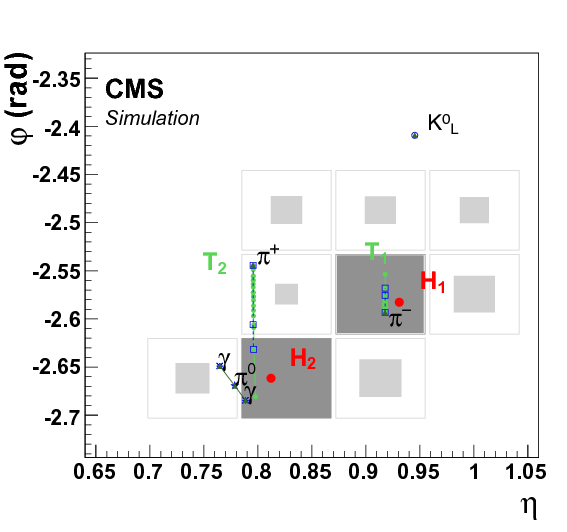
\includegraphics[width=0.49\textwidth]{figures/event_reconstruction/PF_HCAL.png}
  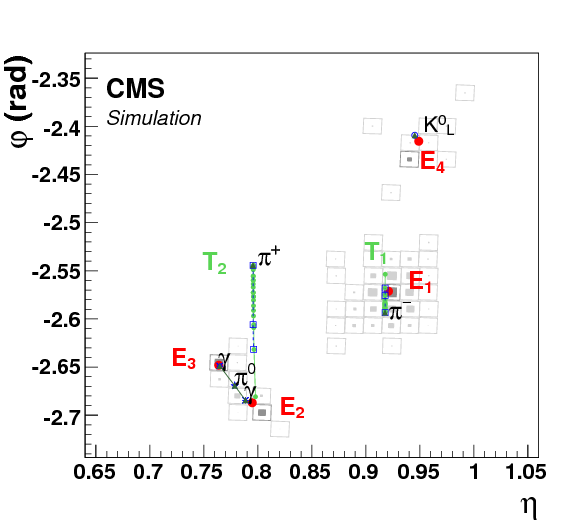
\includegraphics[width=0.49\textwidth]{figures/event_reconstruction/PF_ECAL.png}
    \caption{The $\eta-\phi$ views of calorimeter clusters generated by a five-particle jet in the HCAL (left) and in the ECAL (right). The squares correspond to calorimeter cells, where the inner area is proportional to the logarithm of the cell energy. Cluster seeds are depicted in dark gray. The dotted blue lines correspond to the simulated particle trajectories, while the green lines correspond to charged tracks reconstructed in the tracker~\cite{1748-0221-12-10-P10003}.}
    \label{fig:objreco:caloclustering}
\end{figure} 


\subsection{Particle Flow identification}

\subsubsection{The link algorithm}

The link algorithm is the algorithm responsible for combining the particle flow elements from different subdetectors.
It can test any pair of elements in the event based on specific requirements depending on the nature of the element, but is restricted to the nearest neighbors in the $\eta-\phi$ plane.
The outputs of the link algorithm are so-called \textit{PF blocks} of linked elements, either directly linked or linked through having common elements.
\begin{itemize}
  \item \textbf{Inner track - calorimeter cluster link:} The track is interpolated from its last hit, through the preshower layers, the ECAL, and ending in the HCAL at a nuclear interaction length depth of 1. A link is made if the track is within the cluster areas, where the area is enlarged by up to a cell in each direction to account for detector gaps. In case several ECAL/HCAL clusters are linked to the same track, only the one with the smallest distance in $\eta-\phi$ is kept.

\item \textbf{Calorimeter cluster - cluster link:} A link between ECAL and HCAL clusters, as well as between ECAL and preshower clusters,
is made when the cluster position of the more granular calorimeter is within the cluster envelope of the less granular calorimeter. If there are overlapping links, the one with the smallest distance is kept.

\item \textbf{Inner tracker - muon chamber link:} This procedure is described in Section~\ref{subsub:objreco:muontracking}.
\end{itemize}

\noindent For each PF block, the reconstruction proceeds in the following order. First, muons are reconstructed and their corresponding PF elements removed from the PF block. This is followed by the reconstruction and subsequent removal of electrons and energetic photons. Finally, neutral and charged hadrons are reconstructed.

\subsubsection{Muons}
\label{sec:objreco:muons}
First, isolated global muons are selected by requiring the sum of track \PT and calorimeter energy deposits within a cone of $\Delta R = 0.3$ and not belonging to the muon track, to be smaller than 10 \% of the muon \PT.
If the muons are non-isolated, they are required to pass the tight muon requirement~\cite{1748-0221-7-10-P10002} and have at least three matching track segments in the muon detector or have matched calorimeter deposits compatible with being a minimum ionizing particle.
Muons failing both the requirements above are kept if their standalone muon track is of high quality and have a lot of hits in the muon detectors, otherwise they are discarded.
The muon momentum is defined from the inner tracker measurement if the muon \PT is less than 200 \GeV. Otherwise, it is chosen according to the track fit with the smallest $\chi^2$ probability. \newline

Muons used in this thesis are required to pass an isolation requirement in order to suppress the background from QCD multijet events where jet constituents are identified as muons. For this, a cone of radius $\Delta R = 0.3$ is constructed around the muon direction. The isolation parameter is defined as the scalar sum of the transverse momenta of all additional reconstructed tracks within the cone, divided by the muon \PT{}. Muon candidates with an isolation parameter less
than 0.1 are considered isolated and are used for further analysis. \newline
Further, the following selection criteria are applied:
\begin{itemize}
  \itemsep0em 
  \item the $\chi^2$ of the global muon track fit must be less than 10;
  \item at least one muon-chamber hit is included in the global-muon track fit and the global muon track fit must include at least one muon chamber hit;
  \item muon segments in at least two of the muon stations must be matched to the muon tracker track;  
  \item the inner tracker track must be no more than 2 millimeters from the primary vertex in the xy plane and no more than 5 millimeters in the longitudinal direction;
 \item at least one hit in the pixel detector;
 \item at least six layers of the inner tracker must contain hits; and
 \item at least three matching track segments must be found in the
muon detectors
\end{itemize}


\subsubsection{Electrons}
\label{sec:objreco:electrons}
The electrons are seeded from a GSF track, as described in Section~\ref{subsub:objreco:electrontracking}. To differentiate electrons from charged hadrons, the energy deposit in the HCAL within a distance of 0.15 in the $\eta-\phi$ plane of the supercluster is required to be less than 10 \% of that of the supercluster. The electron candidate must further pass a requirement on the output of a dedicated electron-identification BDT, using inputs such as track-cluster distance, track $\chi^2$, and number of hits as input.  In this step, isolated photons are also reconstructed, seeded from ECAL superclusters with $|E_T>10 \GeV|$ and no link to a GSF track.
All the tracks and calorimeter deposits used to reconstruct electrons and isolated photons are further removed from the list of PF blocks. \newline
Only electrons passing certain quality requirements as listed in Table~\ref{tab:objreco:HEEP} are used in this thesis, with the following variable definitions:
\begin{itemize}
\itemsep-1em 
\item \textbf{$E_T$:} The supercluster energy $(x \sin(\theta_{track}))$, where $\theta_{track}$ is the polar angle of the electron track as measured in the inner tracker layer and extrapolated to the interaction vertex. \newline
\item \textbf{$\eta^{sc}$:} $\eta$ of the electron supercluster.\newline
\item \textbf{isEcalDriven}: The electron is found through ECAL requirements rather than through Particle Flow and the tracker.\newline
\item \textbf{$\Delta \eta_{in}^{seed}$:} difference in $\eta$ between the track position as measured in the inner layer and extrapolated to the interaction vertex and then to the calorimeter, and the $\eta$ of the supercluster. \newline
\item \textbf{$\Delta\phi_{in}$:} difference in $\phi$ bbetween the track position as measured in the inner layer and extrapolated to the interaction vertex and then to the calorimeter, and the $\phi$ of the supercluster. \newline
\item \textbf{H/E:} Ratio of hadronic energy in the calorimeter towers, within a cone of radius 0.15 centered at the electron's calorimeter position to the electromagnetic energy of the supercluster.\newline
\item \textbf{$\sigma_{i \eta i \eta}$:} Measure of the energy spread in $\eta$ in units of crystals of electron energy in a $5 \times 5$ block centered on the seed crystal.\newline
\item \textbf{ECAL Isolation:} The transverse electromagnetic energy of all reconstructed hits (with $E > 0.08 \GeV$) in a cone of radius 0.3 centered at the electron's calorimeter position, excluding those in an inner cone with a radius of 3 crystals and an $\eta$ strip with a width of 3 crystals.\newline
\item \textbf{Hadronic Depth Isolation:} Defined as the transverse depth of the hadronic energy in the HCAL inside a cone of 0.3 centered on the electron calorimeter position, excluding towers in a cone of 0.15 radius.\newline
\item \textbf{Track \PT Isolation:} The sum \PT of the tracks in a $\Delta R$ cone of 0.04 to 0.3, excluding an $\eta$ region of 0.015.\newline
\item \textbf{$d_{xy}$:} Transverse distance between the electron track and the primary vertex.\newline
\end{itemize}

\begin{table}[h!]
\begin{center}
  \footnotesize
\begin{tabular}{l|c|c}
 Variable  &  Barrel  &  Endcap  \\
 \hline
 $E_{T}$                            &  $>$ 35 \GeV                                                &  $>$ 35 \GeV                                         \\
 $\eta$ range                       &  $|\eta_{sc}|< 1.4442$                                      &  $1.566<\eta_{sc} < 2.5$                             \\
 isEcalDriven                       &  yes                                                        &  yes                                                 \\
 $\Delta \eta_{in}^{seed}$          &  $< 0.004$                                                  &  $< 0.006$                                           \\
 $\Delta\phi_{in}$                  &  $< 0.06$                                                   &  $< 0.06$                                            \\
 H/E                                &  $<1/E + 0.05$                                              &  $< 5/E + 0.05$                                      \\
 full 5x5 $\sigma_{i \eta i \eta}$  &  n/a                                                        &  $<0.03$                                             \\
 full 5x5 $E^{2x5}/E^{5x5}$         & $>0.94$ OR $E^{1x5}/E^{5x5}> 0.83$                          &  n/a                                                 \\
 \hline
 EM$+$Had. Depth Iso.               &  $ < 2+0.03 \times E_T + 0.28 \times \rho$                  & $E_T < 50 \GeV$: $< 2.5+0.28 \times \rho$        \\
                                    &                                                             & else: $<2.5+0.03 \times (E_T-50) + 0.28 \times \rho$ \\
 \hline
 Track \PT iso.                     & $E_T < 100 \GeV: <5 + 1.5 \times \rho$   &  $<5 + 0.5 \times \rho$                              \\
                                    & else:  $<5 + 1.5 \times \rho$                               &                                                      \\
 \hline
 Inner Layer Lost Hits              &  $\leq 1$                                                   &  $\leq 1$                                            \\
 $d_{xy}$                           &  $<0.02$                                                    &  $<0.05$                                             \\
\hline
\end{tabular}
\caption{Summary of the electron requirements applied to all electrons used in this analysis.}
\label{tab:objreco:HEEP}
\end{center}
\end{table}


\subsubsection{Hadrons}
Finally, after the removal of muons and electrons, the remaining hadrons and non-isolated photons are identified. HCAL clusters with no track link are defined as neutral hadrons, while ECAL clusters with no track link are defined as photons (photons are exclusively associated to the ECAL deposits since neutral hadrons leave only 3 \% of their energy in the ECAL).
The remaining HCAL clusters are then linked to one or more tracks from the inner tracker. In order to determine the particle content within a cluster, the sum of track momenta and the calorimeter energy is compared. If the calorimeter energy is compatible with the sum of track momenta, a particle for each track is inferred, with its corresponding energy taken from the track momentum. If the calorimeter energy is larger than the sum of track momenta, a photon or a neutral hadron is added, together with one charged hadron for each track within the cluster area.

\subsubsection{Missing transverse energy}
Neutrinos (and other predicted, non-SM weakly interacting particles) do not interact in the detector and are instead inferred from the presence of a momentum imbalance in the detectors transverse plane. The missing transverse momentum is defined as the negative \PT vector sum of all reconstructed PF candidates in the event,
\begin{equation}
\ptvecmiss = -\sum_{i}^{N}{\vec p}_{\mathrm{T},i},
\end{equation}
and its magnitude, $|\ptvecmiss|$, is referred to as the missing transverse energy \ETmiss (which is used as a proxy for the neutrino \PT).
 
\section{Pile-up removal}

Particles originating from proton-proton interactions not associated with the hardest primary vertex, are denoted as pileup events.
These distort observables of interest from the hard scattering event and must be mitigated through dedicated pileup removal techniques.

\subsection{Charged Hadron Subtraction}
\label{subsub:objreco:chs}
As mentioned previously, primary vertices are reconstructed using tracks from charged hadrons. If a primary vertex does not correspond to the hard scattering vertex of the event, the charged hadrons (as reconstructed through Particle Flow) associated to this vertex (called a pileup vertex) are removed from the event collection of particles and will not participate in any further object reconstruction. This method is denoted charged hadron subtraction (CHS).

\subsection{Pile up per particle identification (PUPPI)}
\label{subsub:objreco:puppi}
CHS was the default pileup removal algorithm in CMS until very recently. In 2014, a new pileup removal algorithm with improved performance was proposed; the pileup per particle identification (PUPPI)~\cite{Bertolini2014} algorithm.
PUPPI uses a combination of local shape information, event pileup properties, and tracking information to compute a weight describing the degree to which a given particle is likely to arise from pileup.
First, a variable denoted $\alpha$ is computed based on the difference between soft radiation coming from pileup and the harder collinear QCD pattern. The shape of $\alpha$ for charged particles is then used as a proxy for all pileup particles and is used on an event-by-event basis to calculate a weight for each particle. This weight in turn describes the degree to which particles are pileup-like and are used to rescale the particle four-momenta.

The shape variable for a given particle $i$ is defined as

\begin{equation}
  \alpha_i = \log \sum_{\substack{j \in \mathrm{Ch,PV} \\ j \neq i}} \left(\frac{p_{T,j}}{\Delta R_{ij}}\right)^{2} \Theta(R_0 - \Delta R_{ij}),
\end{equation}

where $\Theta$ is the step function and $j$ refers to the neighboring charged particles from the primary vertex within a cone of radius $R_0=0.4$. Charged particles are defined as coming from the primary vertex if they are associated to the leading vertex of the event or are within a distance of $d_z < $0.3~\cm from the leading vertex. 

In order to determine the probability that a particle comes from pileup, a $\chi^{2}$ calculation is performed. The probability is defined as

\begin{equation}
\chi^{2}_{i} = \frac{(\alpha_i -  \bar{\alpha}_{PU})^{2}}{RMS_{PU}^{2}},
\end{equation}

where $\bar{\alpha}_{PU}$ is the median value of the $\alpha_i$ distribution for pileup particles in the given event and $RMS_{PU}$ is its RMS.

Each particle (neutral and charged) is then assigned a weight $w_i = F_{\chi^2,NDF=1}(\chi^2_i)$, where $F_{\chi^2,NDF=1}$ is the cumulative distribution function of the $\chi^2$ distribution with one degree of freedom. Particles with $w_{i}<0.01$ are rejected.
In addition, a cut on the weighted \PT of neutral particles of $w_{i} \cdot p_{T,i} >  (A + B \cdot N_{PV})$ \GeV is applied, where $N_{PV}$ correspond to the number of reconstructed vertices in the event and A and B are tunable parameters. 

The performance of the PUPPI algorithm compared to CHS for jet observables is shown in Figure~\ref{fig:objreco:puppi}.

\begin{figure}[h] 
    \centering
    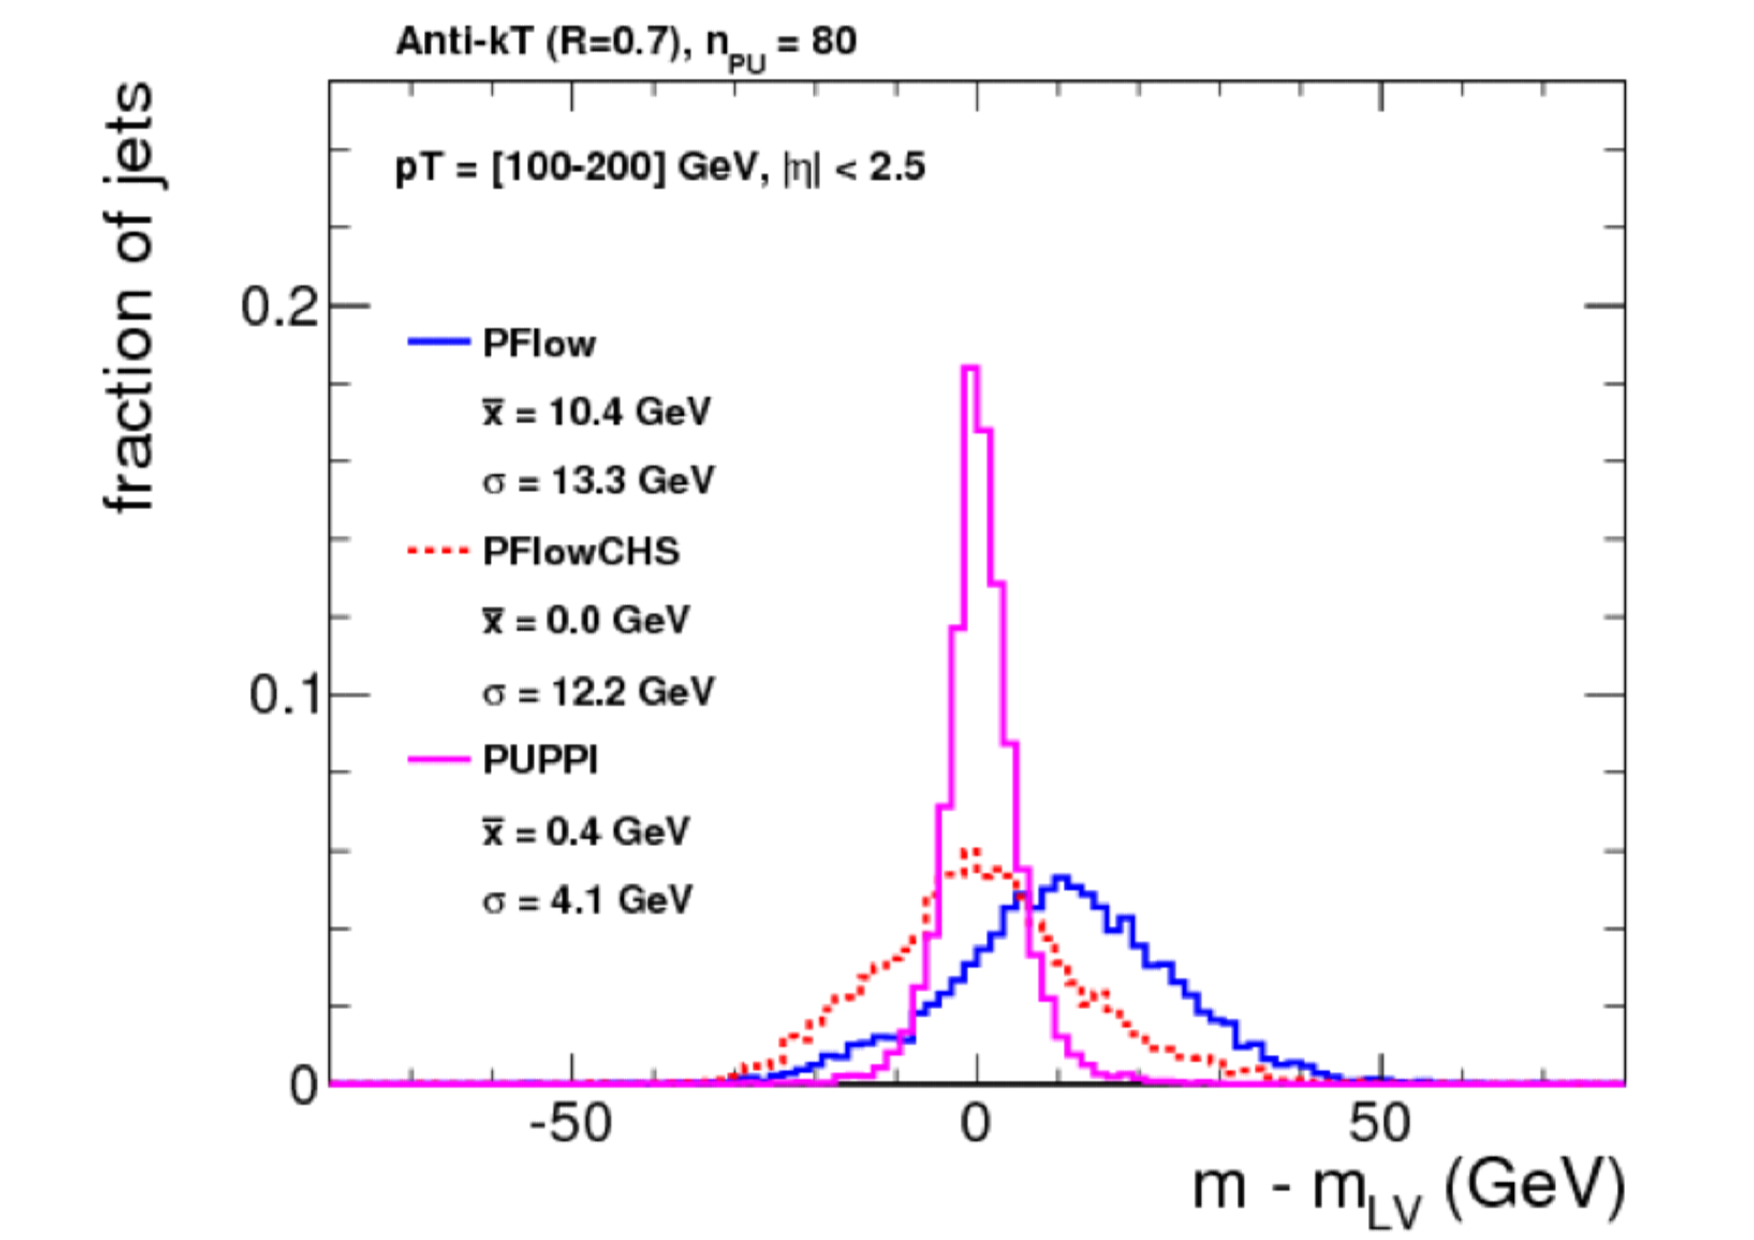
\includegraphics[height=5cm]{figures/event_reconstruction/puppi_mres_hiPt.pdf}
    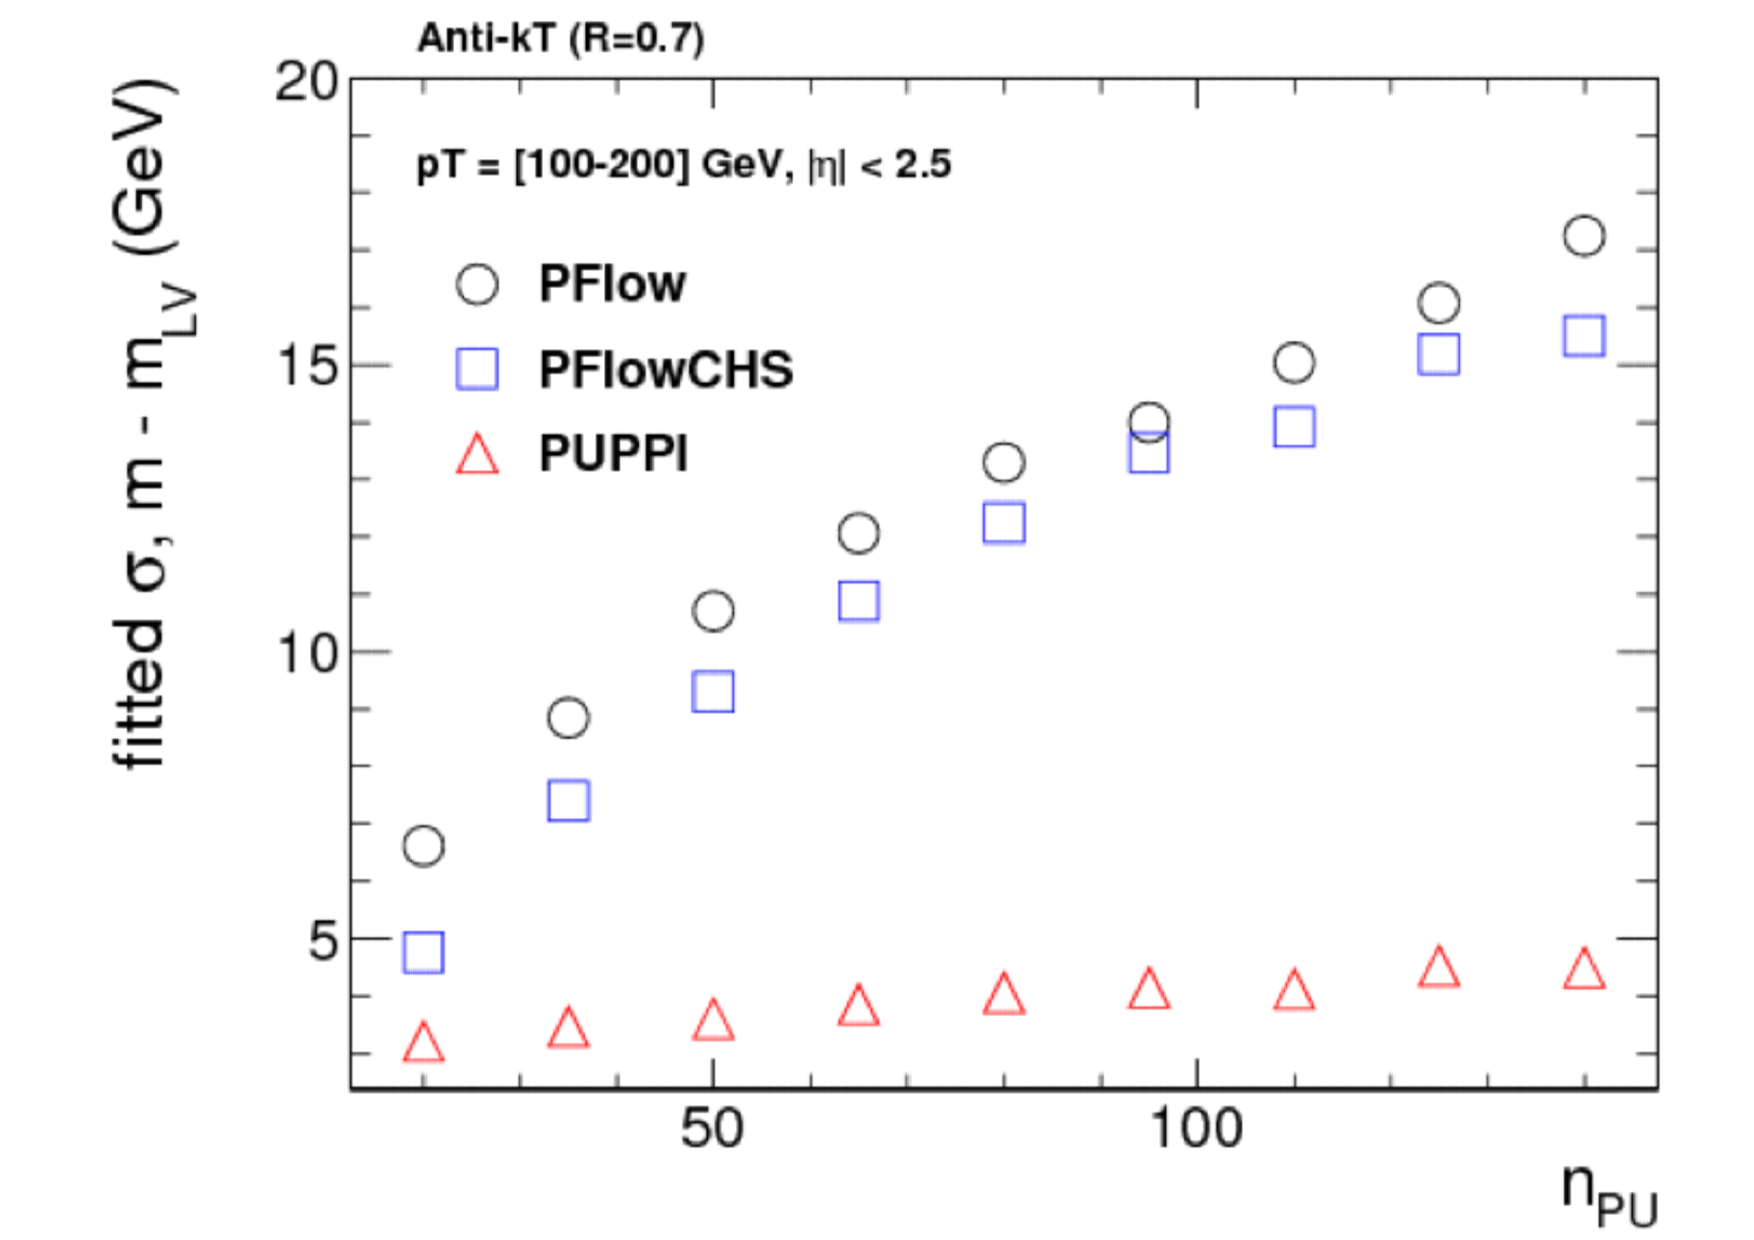
\includegraphics[height=5cm]{figures/event_reconstruction/puppi_mresVsPu.pdf}\\
    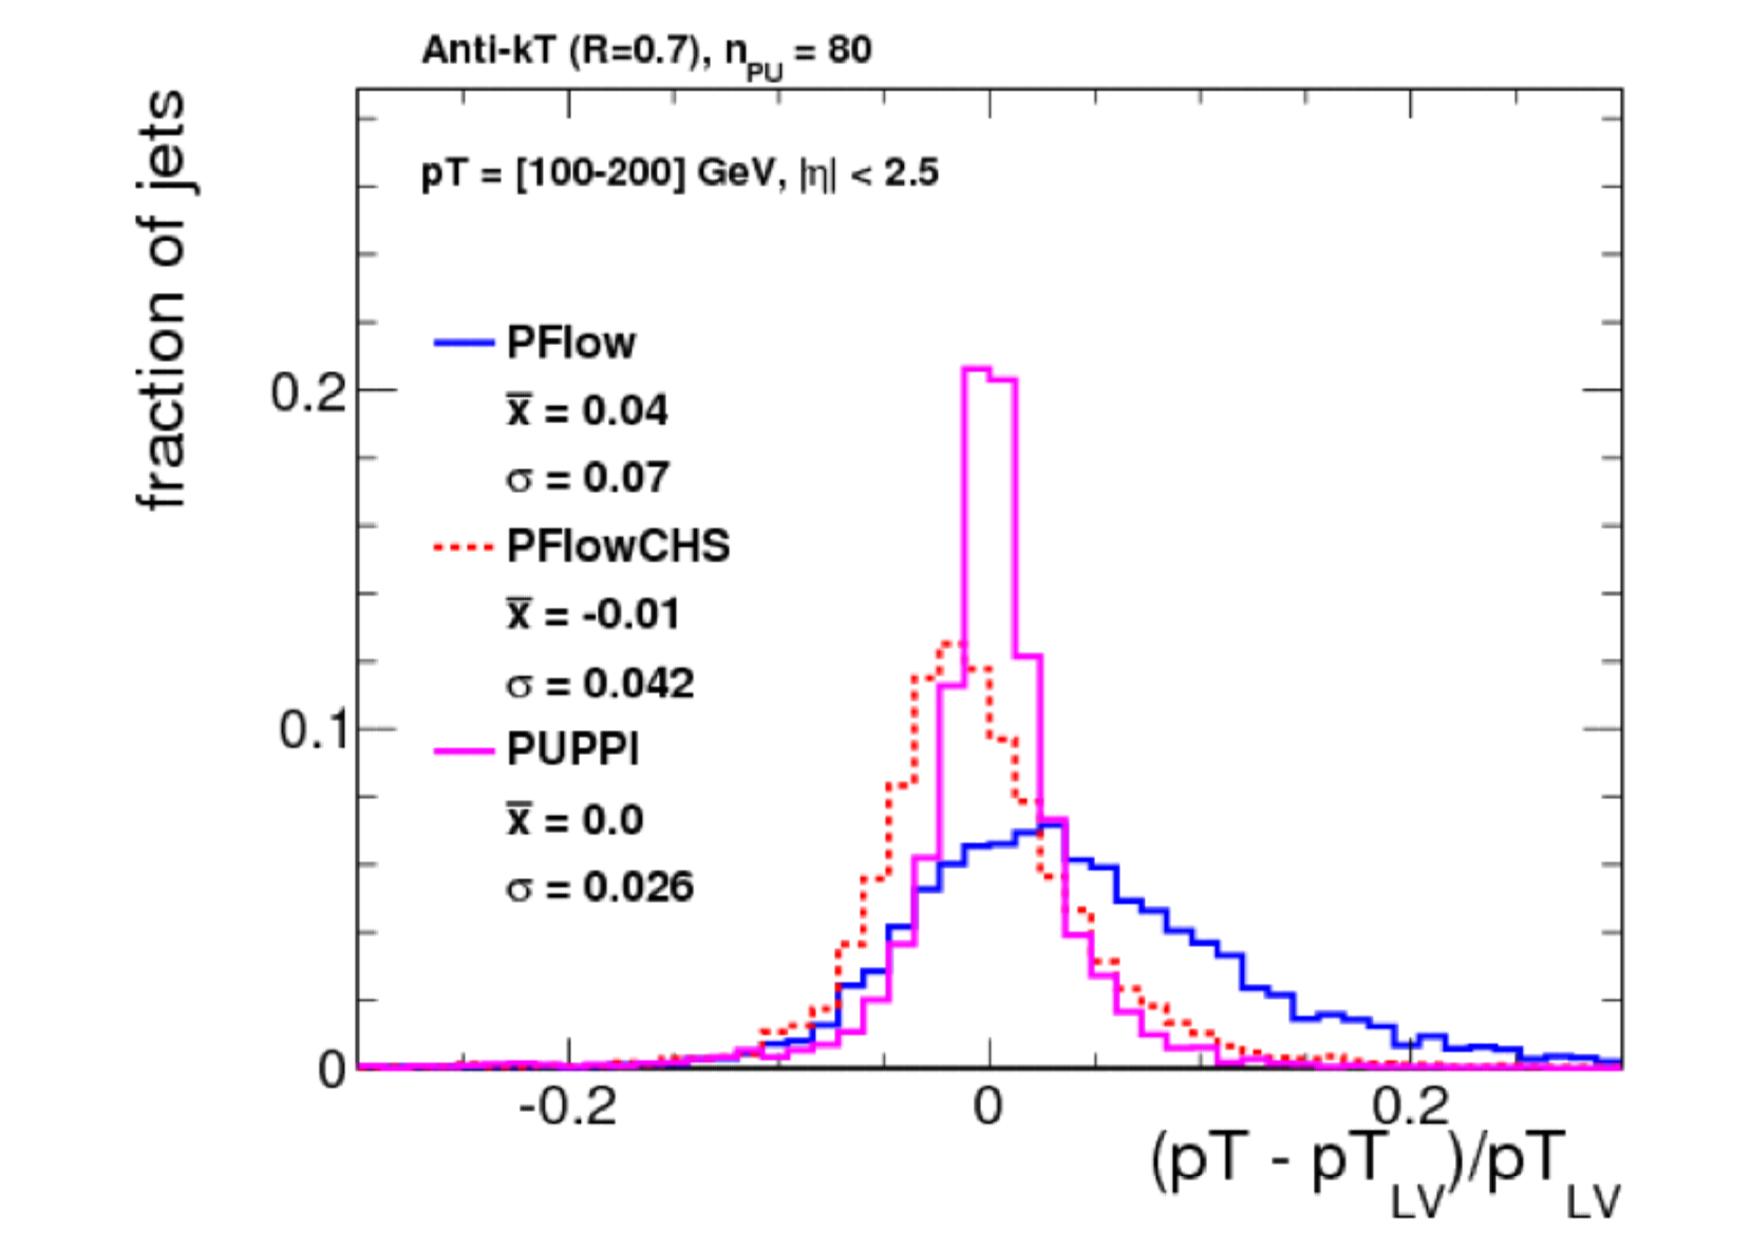
\includegraphics[height=5cm]{figures/event_reconstruction/puppi_ptres_hiPt.pdf}
    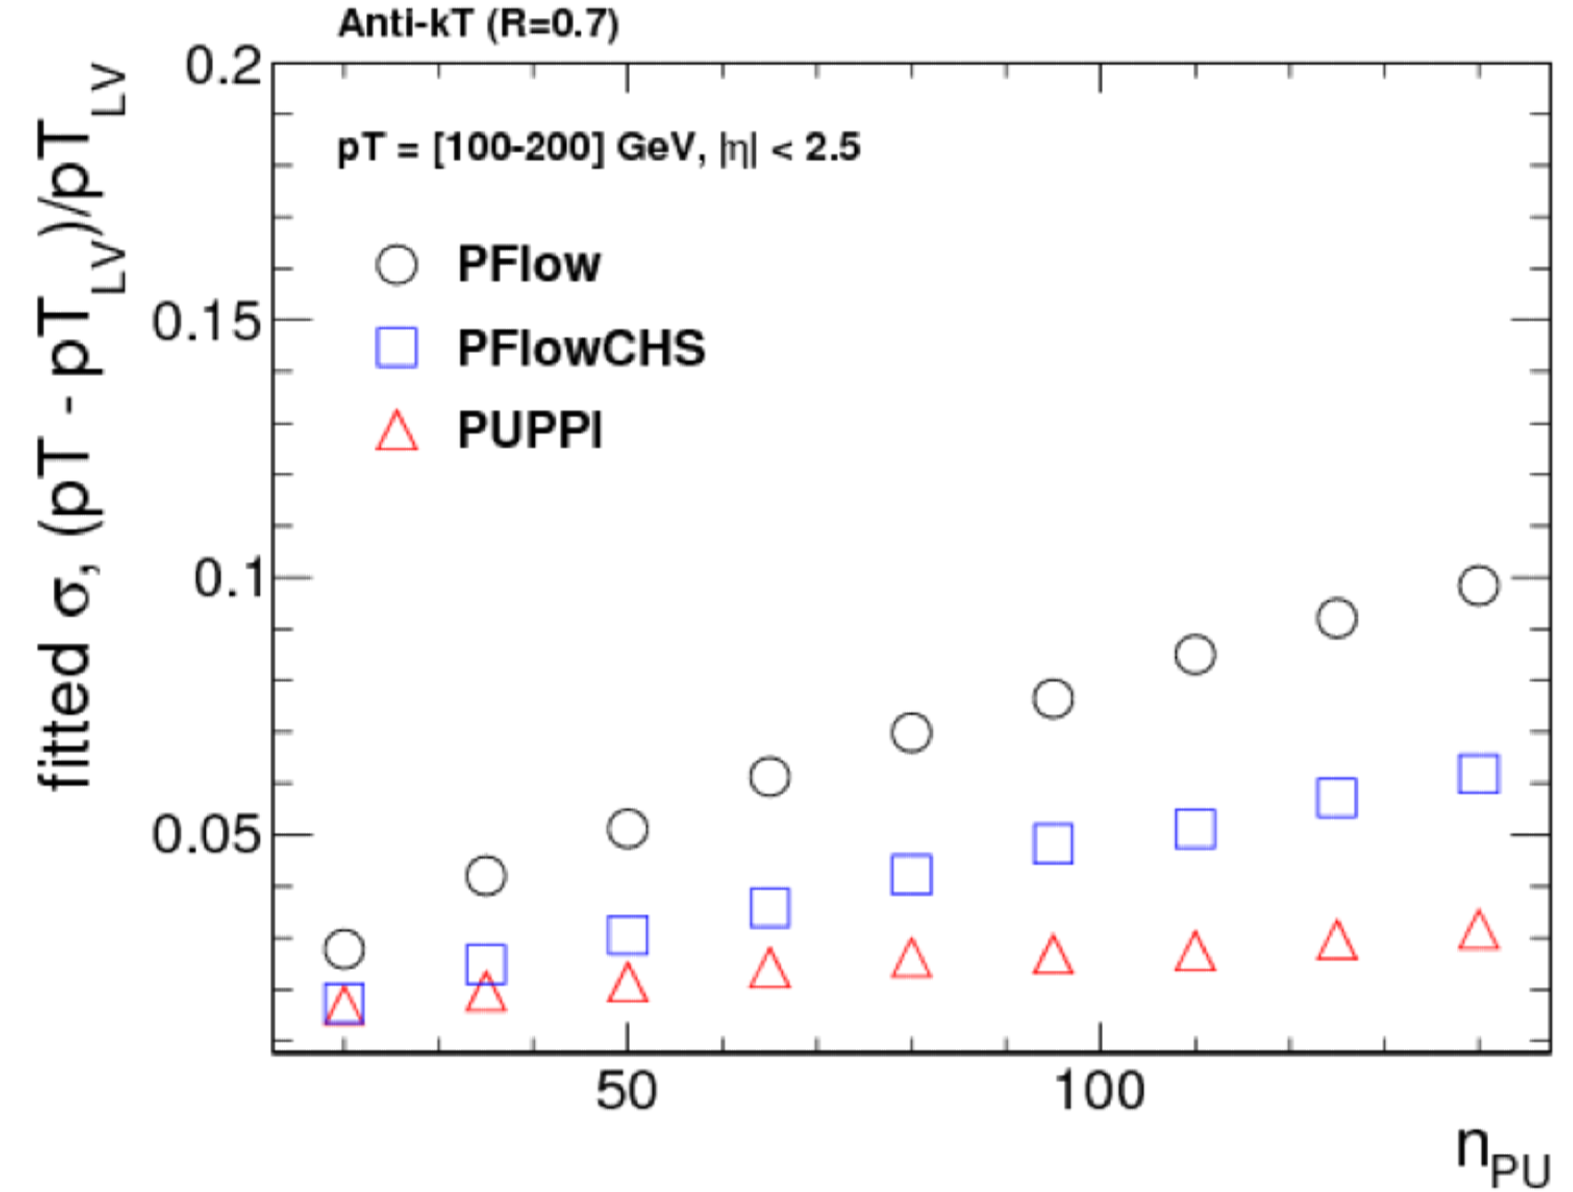
\includegraphics[height=5cm]{figures/event_reconstruction/puppi_ptresVsPu.pdf}
    \caption{The mass (top) and \PT (bottom) resolution comparing PF-only (blue), PF+CHS (red) and PUPPI (pink) jets. The absolute resolution (left) as well as the resolution as a function of the number of reconstructed primary vertices in the event (right) is shown~\cite{Bertolini2014}.}
    \label{fig:objreco:puppi}
\end{figure}

The top row shows the absolute mass resolution (left), as well as the mass resolution as a function of $N_{PV}$ for CHS jets (red) and PUPPI (pink) jets. The bottom row shows the corresponding quantities but for jet transverse momentum. A significantly better resolution on jet observables can be achieved using PUPPI as compared to CHS.

\section{Jet reconstruction}
\label{sec:objreco:jets}
As explained in Section~\ref{sec:theory:qcd}, quarks and gluons are never themselves visible in a detector. Within $10^{-23}$ seconds, the timescale of strong interactions, they fragment and hadronize into a collimated spray of hadrons, a so-called jet. In order to infer the properties of the original parton generating the jet, the properties of the full particle spray needs to be evaluated.
Combining these particles algorithmically is non-trivial, and several algorithms jet-clustering algorithms exist.
These provide a set of rules for grouping particles together into jets and are usually based on certain distance requirements between particles as well as rules for how to recombine their momenta.
Thanks to Particle Flow, objects like charged hadrons, neutral hadrons and photons, together with their estimated energy and direction, are already defined and jet clustering in CMS therefore consists of associating these particles to one common origin.


\subsection{Jet clustering}

The most common jet clustering algorithms used in hadron colliders are the Cambridge/Aachen algorithm~\cite{Dokshitzer:1997in}, the \kt algorithm~\cite{Ellis:1993tq} and the anti-\kt algorithm~\cite{Cacciari:2008gp}. These are all sequential recombination algorithms, meaning they systematically go through each particle pair in the event and recombines them into one particle if the combination satisfies certain criteria. The rules, shared by all three algorithms, are as follows:
\begin{enumerate}
  \itemsep0em 
\item For each pair of particles $i$ and $j$, compute the longitudinally invariant distances
  \begin{align}
    \label{eq:objreco:jetclustering1}  
  d_{ij} &= \textrm{min}(p_{ti}^{2p},p_{tj}^{2p})\frac{\Delta R^2_{ij}}{R^2} \quad \textrm{, with } \quad \Delta R^2_{ij}=(\eta_i - \eta_j)^2+(\phi_i - \phi_j)^2 \textrm{, and }\\
  \label{eq:objreco:jetclustering2}  
  d_{iB} &= p_{ti}^{2p},
  \end{align}  
  where $d_{ij}$ is a measure of the relative transverse momenta between the particles, $\Delta R^2_{ij}$ is the distance between them in the $\eta-\phi$ plane (which can be roughly translated into a jet radius), $\Delta R^2$ corresponds to a distance parameter which controls the extension of the jet and $d_{iB}$ is the distance between the particle and the beam. The parameter $p$ is what separates the three algorithms from one another and controls the relative power of energy versus geometrical
scales. For the anti-\kt algorithm, it is defined as $p=-1$; for the \kt algorithm, $p=1$; and in the case of the C/A algorithm, $p=0$. The consequences of these choices are explained in detail below.
  \item Find the minimum distance of $d_{ij}$ and $d_{iB}$.
  \item If this is $d_{ij}$, recombine particles $i$ and $j$ and return to step 1.
  \item If it is $d_{iB}$, the particle $i$ is defined to be a final state jet, and is removed from the list of particles. The algorithm proceeds back to step 1.
  \item Repeat until no particles remain.
\end{enumerate}

\subsubsection{Infrared and collinear safety}
There are two requirements that are extremely important when defining jet algorithms: They must be 1) \textit{infrared} (IR) and 2) \textit{collinear} (C) safe.
\textit{Infrared} safety corresponds to the requirement that if the final state particles are modified by the presence of a soft emission, and there are always soft emission in QCD events (both perturbative and non-perturbative), then the set of hard jets should remain unchanged. This is illustrated by the two left figures in Figure~\ref{fig:objreco:IRC}.

\begin{figure}[h!] 
    \centering
    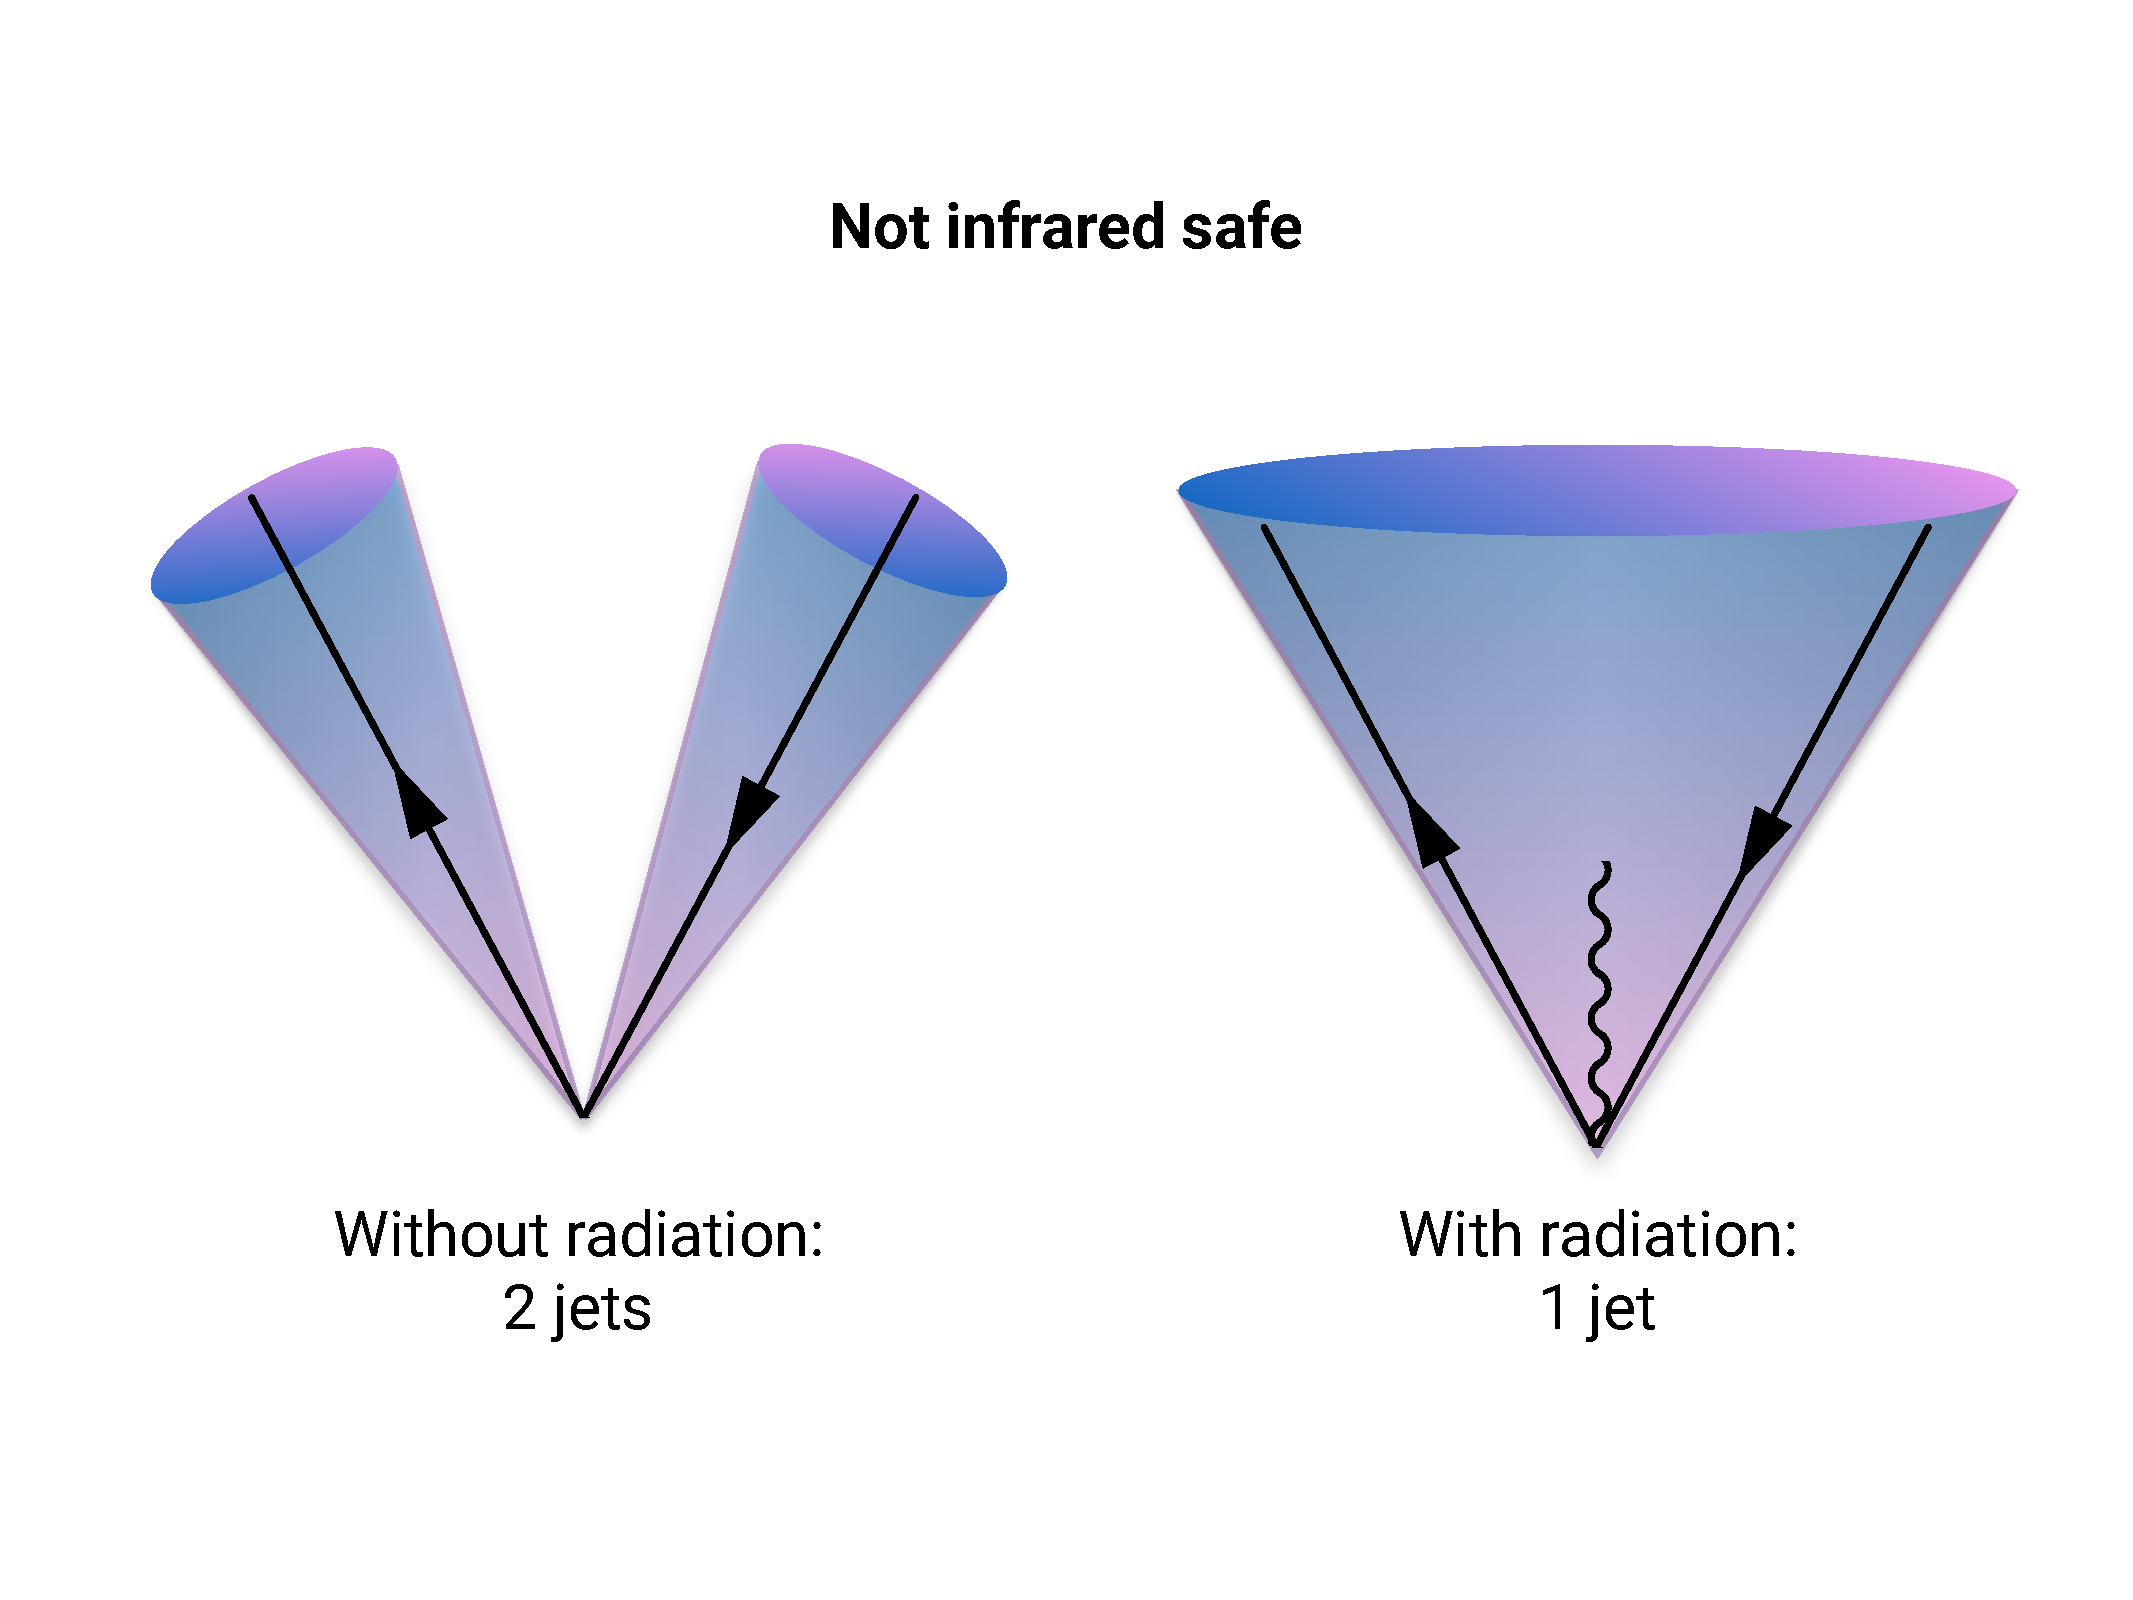
\includegraphics[width=0.49\textwidth]{figures/event_reconstruction/IR_safety.pdf}
    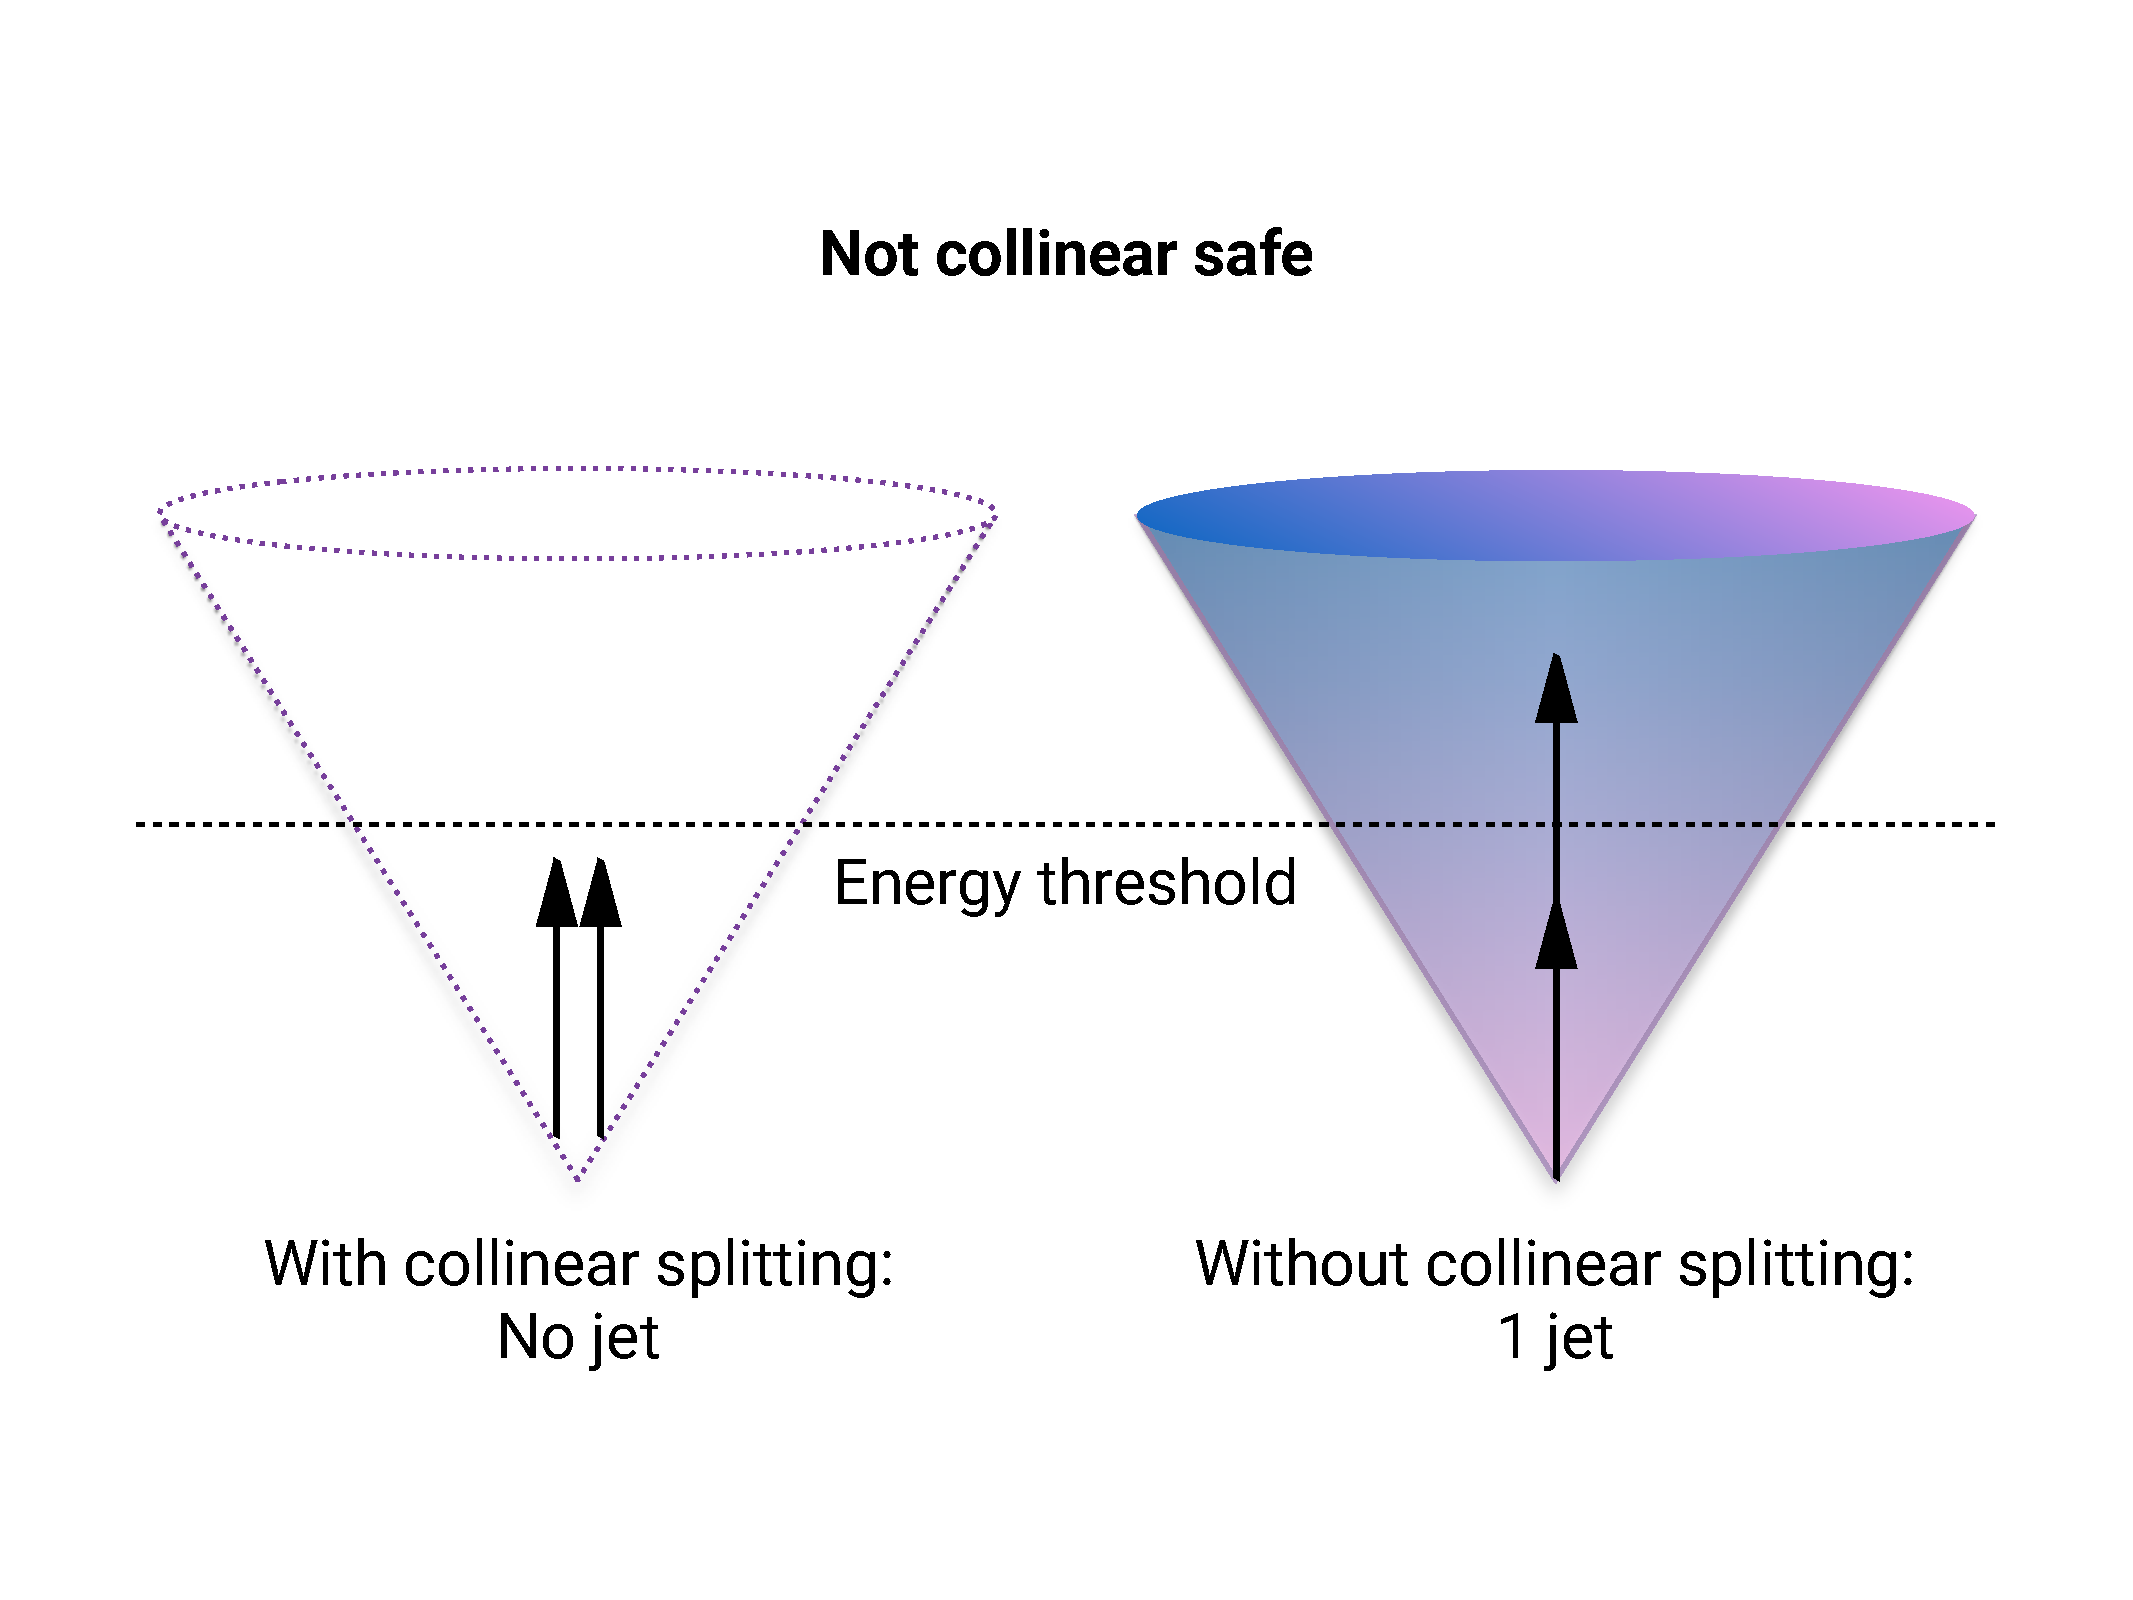
\includegraphics[width=0.49\textwidth]{figures/event_reconstruction/Collinear_safety.pdf}
    \caption{An illustration of what would happen for an infrared (left) and collinear (right) unsafe jet algorithm. If an algorithm is infrared unsafe, the presence of a soft emission changes the jet configuration. If an algorithm is collinear unsafe, then if a parton undergoes a collinear splitting this will change the configuration of the jet.}
    \label{fig:objreco:IRC}
\end{figure}

Here, the algorithm is infrared unsafe: the presence of an additional soft gluon changes the jet configuration from 2 to 1 jets. If an algorithm is \textit{collinear} unsafe, it means that the jet configuration would change if the hard parton undergoes collinear splitting (which a hard parton often does as part of the fragmentation process and which are also part of non-perturbative dynamics, like the decay of highly energetic hadrons). This is shown in the two left figures of Figure~\ref{fig:objreco:IRC}, where a hard parton undergoing collinear splitting fails to be reconstructed due to its daughters being below the energy threshold of the algorithm.


All sequential recombination algorithms are trivially infrared safe.
 
\subsubsection{The \kt algorithm}
The \kt algorithm is the oldest of the sequential recombination algorithms and, due to its $p=1$ definition in Equations~\ref{eq:objreco:jetclustering1} and~\ref{eq:objreco:jetclustering2}, follows the QCD branching structure in both \PT and in angle (in reverse). Soft particles are clustered together first, and the final step is the clustering of the two hardest particles. A consequence of this definition is that there is nothing that keeps arbitrarily soft particles from being defined as jets, and a minimum cut on the jet \PT should be introduced.
Despite several favorable qualities, the \kt algorithm is not the algorithm of choice in most hadron collider experiments due to the irregular jets it produces, a consequence of clustering soft particles first.

\subsubsection{The Cambridge/Aachen algorithm}
The Cambridge/Aachen algorithm, with $p=0$ in Equations~\ref{eq:objreco:jetclustering1} and~\ref{eq:objreco:jetclustering2}, follows the QCD branching structure only in angle as the clustering order is based solely on spatial separation. The simplest of the algorithms, it recombines all pairs close in $\Delta R$ until $\Delta R_{ij} > R$.
The benefits of this is that the clustering history contains information about the presence of any geometrical substructure within a jet, a feature that will become important in Section~\ref{sec:objreco:substructure}.

\subsubsection{The anti-\kt algorithm}
The default jet clustering algorithm in CMS is the anti-\kt algorithm~\cite{Cacciari:2008gp}, which follows the clustering rules in Equations~\ref{eq:objreco:jetclustering1} and~\ref{eq:objreco:jetclustering2} with $p=1$. The algorithm favors the clustering between high \PT particles, and high and low \PT particles first, disfavoring clustering between soft particles. That means the algorithm grows around a hard core, yielding jets with a well-defined cone shaped area. Since the algorithm is infrared- and collinear-safe (IRC safe) and insensitive to the underlying event (parton remnants not from the hard process) and pileup, , it is chosen as the main jet algorithm in CMS. A comparison of the resulting jet area in the $\phi-\eta$ plane after clustering with either \kt, C/A and anti-\kt, is shown in Figure~\ref{fig:objreco:jetalgo_comp}. The z-axis correspond to the parton \PT. One can clearly see that when clustering with the anti-\kt algorithm, the produced jets are circular, with a radius set by $R$, around the hardest parton.

\begin{figure}[h] 
    \centering
    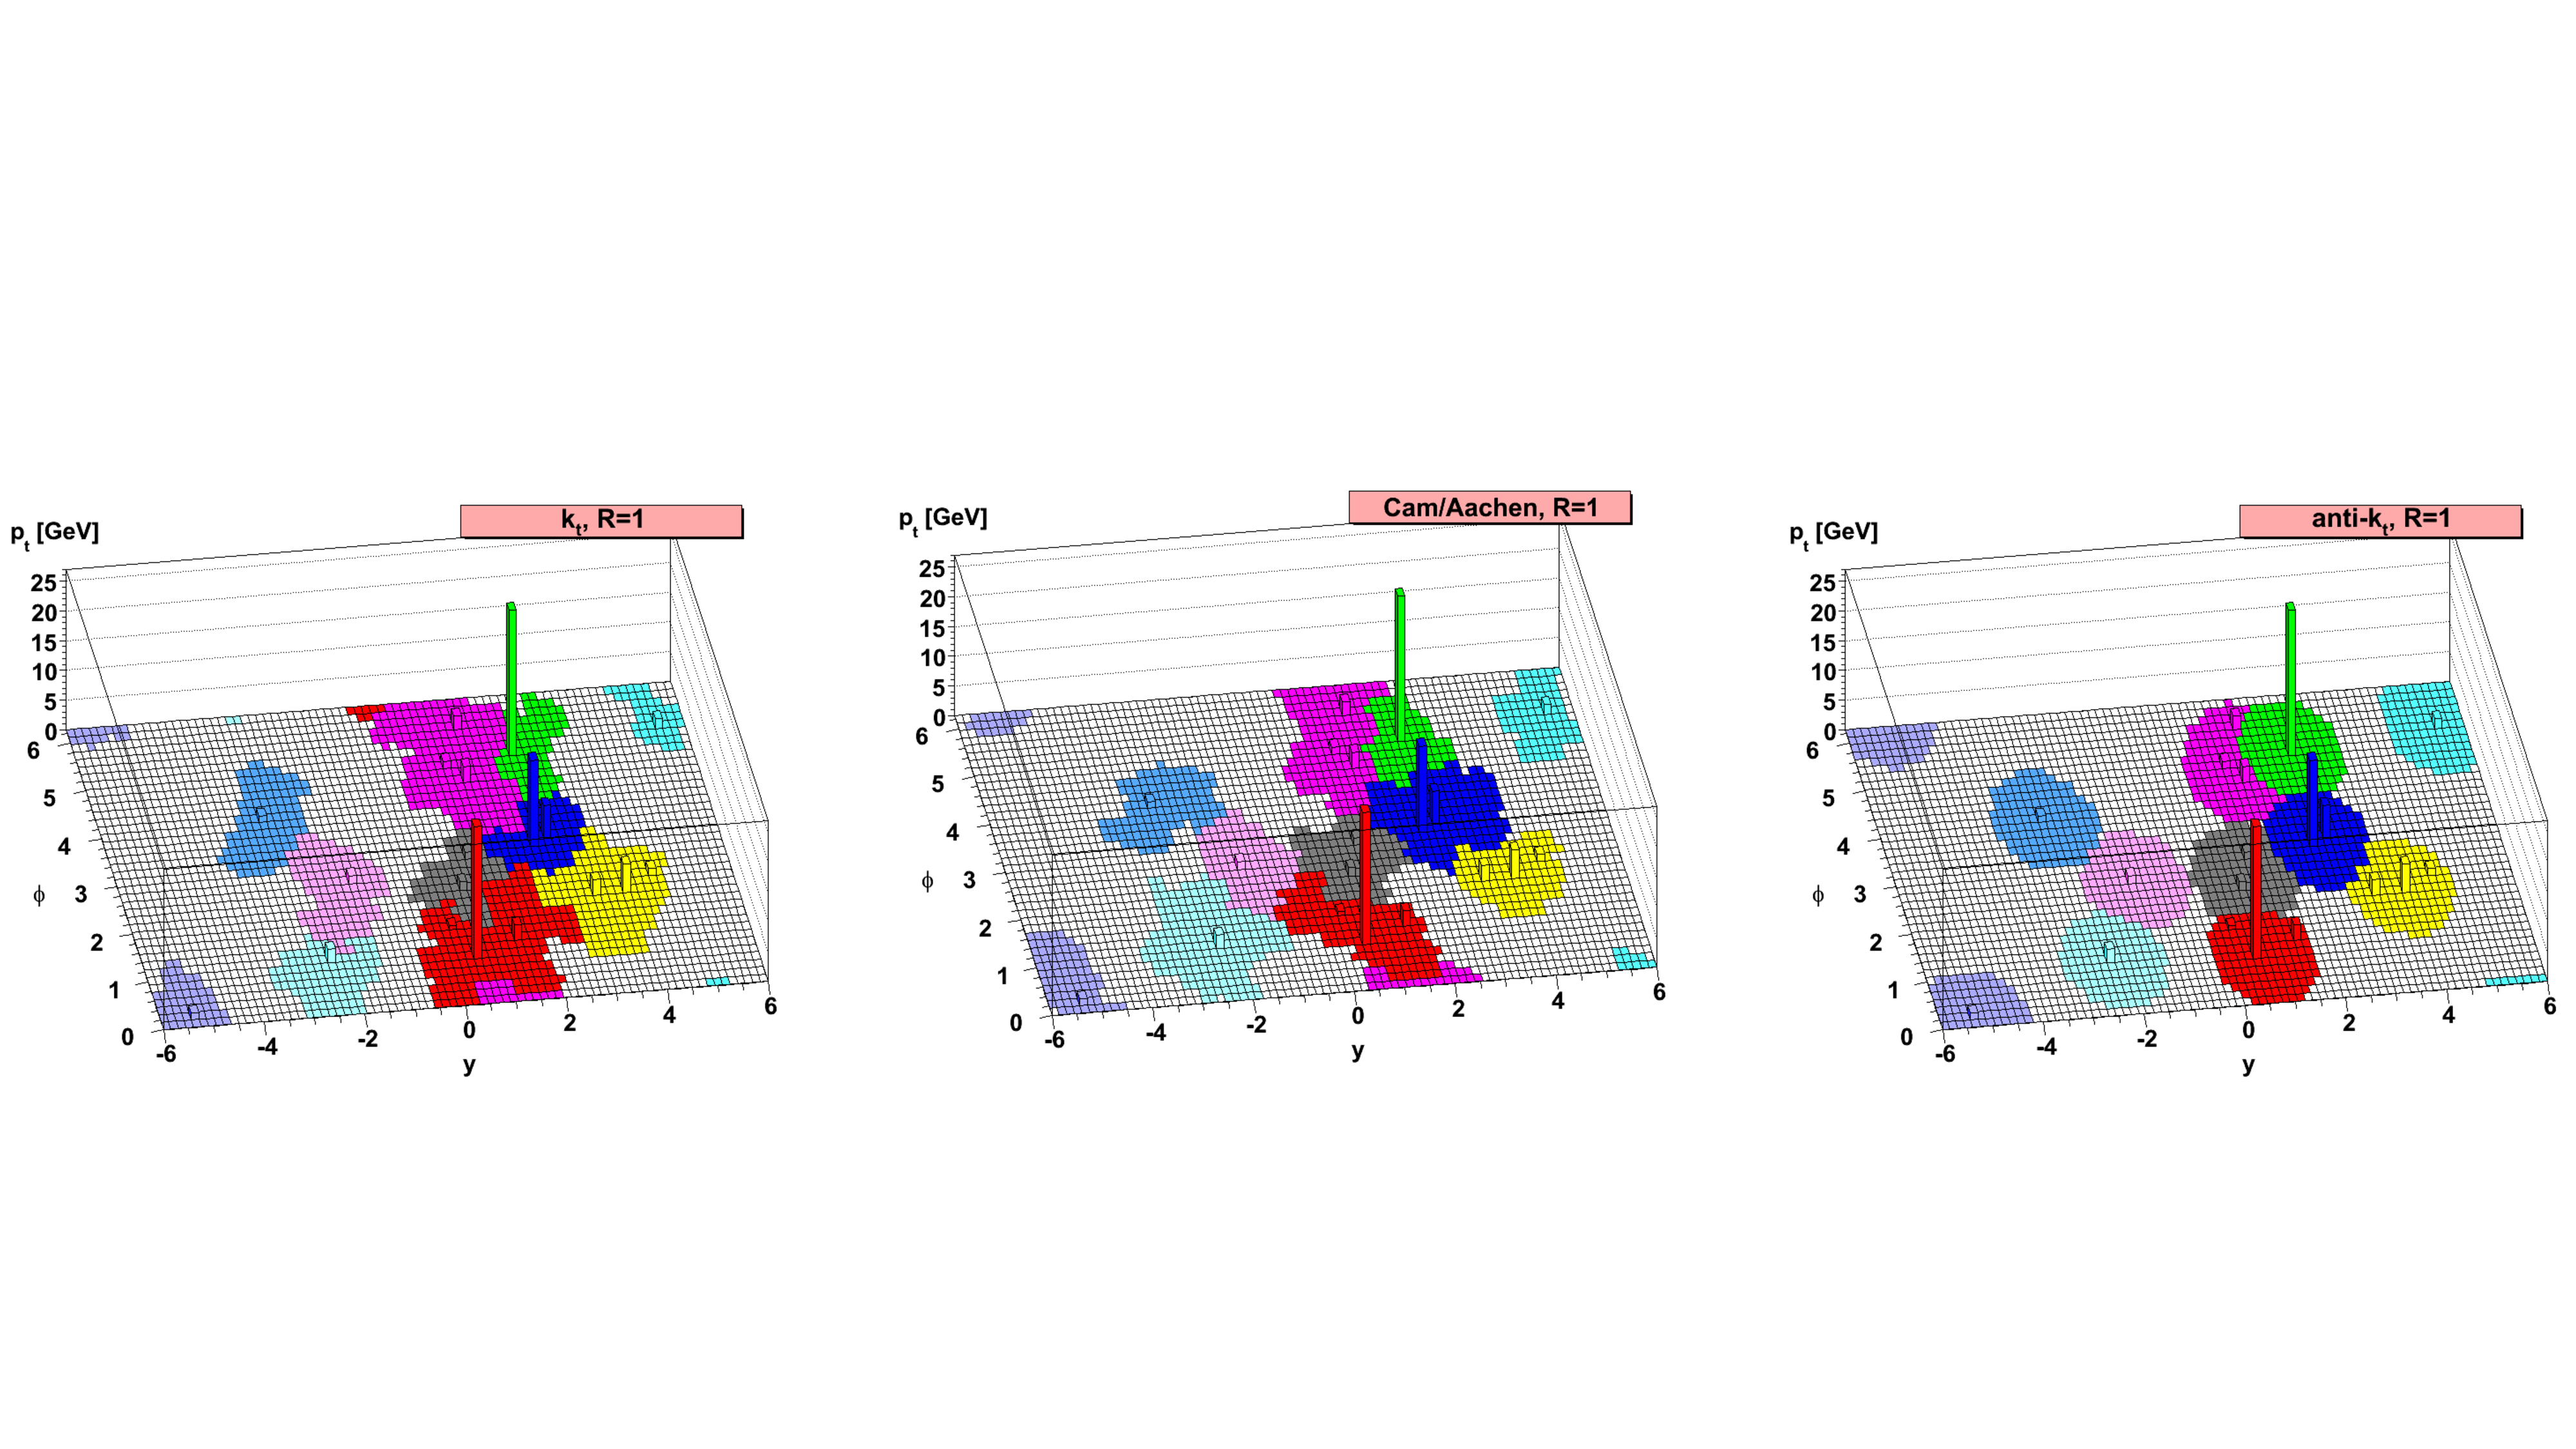
\includegraphics[width=0.99\textwidth]{figures/event_reconstruction/clustering_algos.pdf}
    \caption{A comparison of the resulting jet cone area in the $\phi-\eta-\PT$ plane after clustering the same event with three different jet algorithms: \kt, C/A and anti-\kt. ~\cite{Cacciari:2008gp}}
    \label{fig:objreco:jetalgo_comp}
\end{figure}

\subsection{PF jets in CMS}
Jet algorithms in CMS mainly use the four-vectors of PF candidates as input and a pileup removal algorithm is usually applied before clustering occurs. If using CHS (Section~\ref{subsub:objreco:chs}), charged hadrons not associated to the primary vertex are discarded before clustering. If PUPPI is used (Section~\ref{subsub:objreco:puppi}), all the PF candidates are reweighted based on how likely they are to have originated from pileup. 
For the anti-\kt algorithm, CMS by default uses two jet cone sizes: R=0.4 and R=0.8. Jets with R=0.4, called PFAK4, are used for single-prong jets while the larger R=0.8 jets, PFAK8, are more often used when looking for jets containing multiple hard quarks/gluons in order to contain all the hadronization products.\par
 These jets are further required to pass certain jet identification requirements provided by the JetMET POG~\cite{jetID_JME}, in order to distinguish them from fake jets. All jets used in this analysis are required to pass the \textit{tight ID} requirements which are as follows:
\begin{itemize}
  \itemsep0em 
\item the jet must contain at least two PF constituents;
\item at least one of these constituents must be a charged hadron;
\item the fraction of jet energy coming from neutral hadrons must be $< 0.90$;
\item the fraction of jet energy coming from neutral electromagnetic energy must be $< 0.90$; and
\item the fraction of jet energy coming from charged electromagnetic energy must be $< 0.99$.
\end{itemize} 

\subsection{Jet energy corrections}
\label{sec:objreco:jec}
All jets are further corrected for nonlinearities in $\PT$ and pseudorapidity using standard CMS jet energy corrections (JEC), as described in Ref.~\cite{jme_jinst}. These are intended to bring the measured jet energy closer to the true jet energy by correcting the jet energy scale (JES) and jet energy resolution (JER). The energy corrections are derived in three steps:
\begin{itemize}
  \itemsep0em 
  \item L1: Energy offset corrections intended to remove pileup and electronic noise, both for data and simulation;
  \item L2L3: A relative (L2) and absolute (L3) correction to particle level jet response for simulation only; and
  \item Residual: A correction for data only meant to correct for residual differences between data and simulation.
\end{itemize}

These are illustrated in Figure~\ref{fig:objreco:jec}.

\begin{figure}[h]
    \centering
    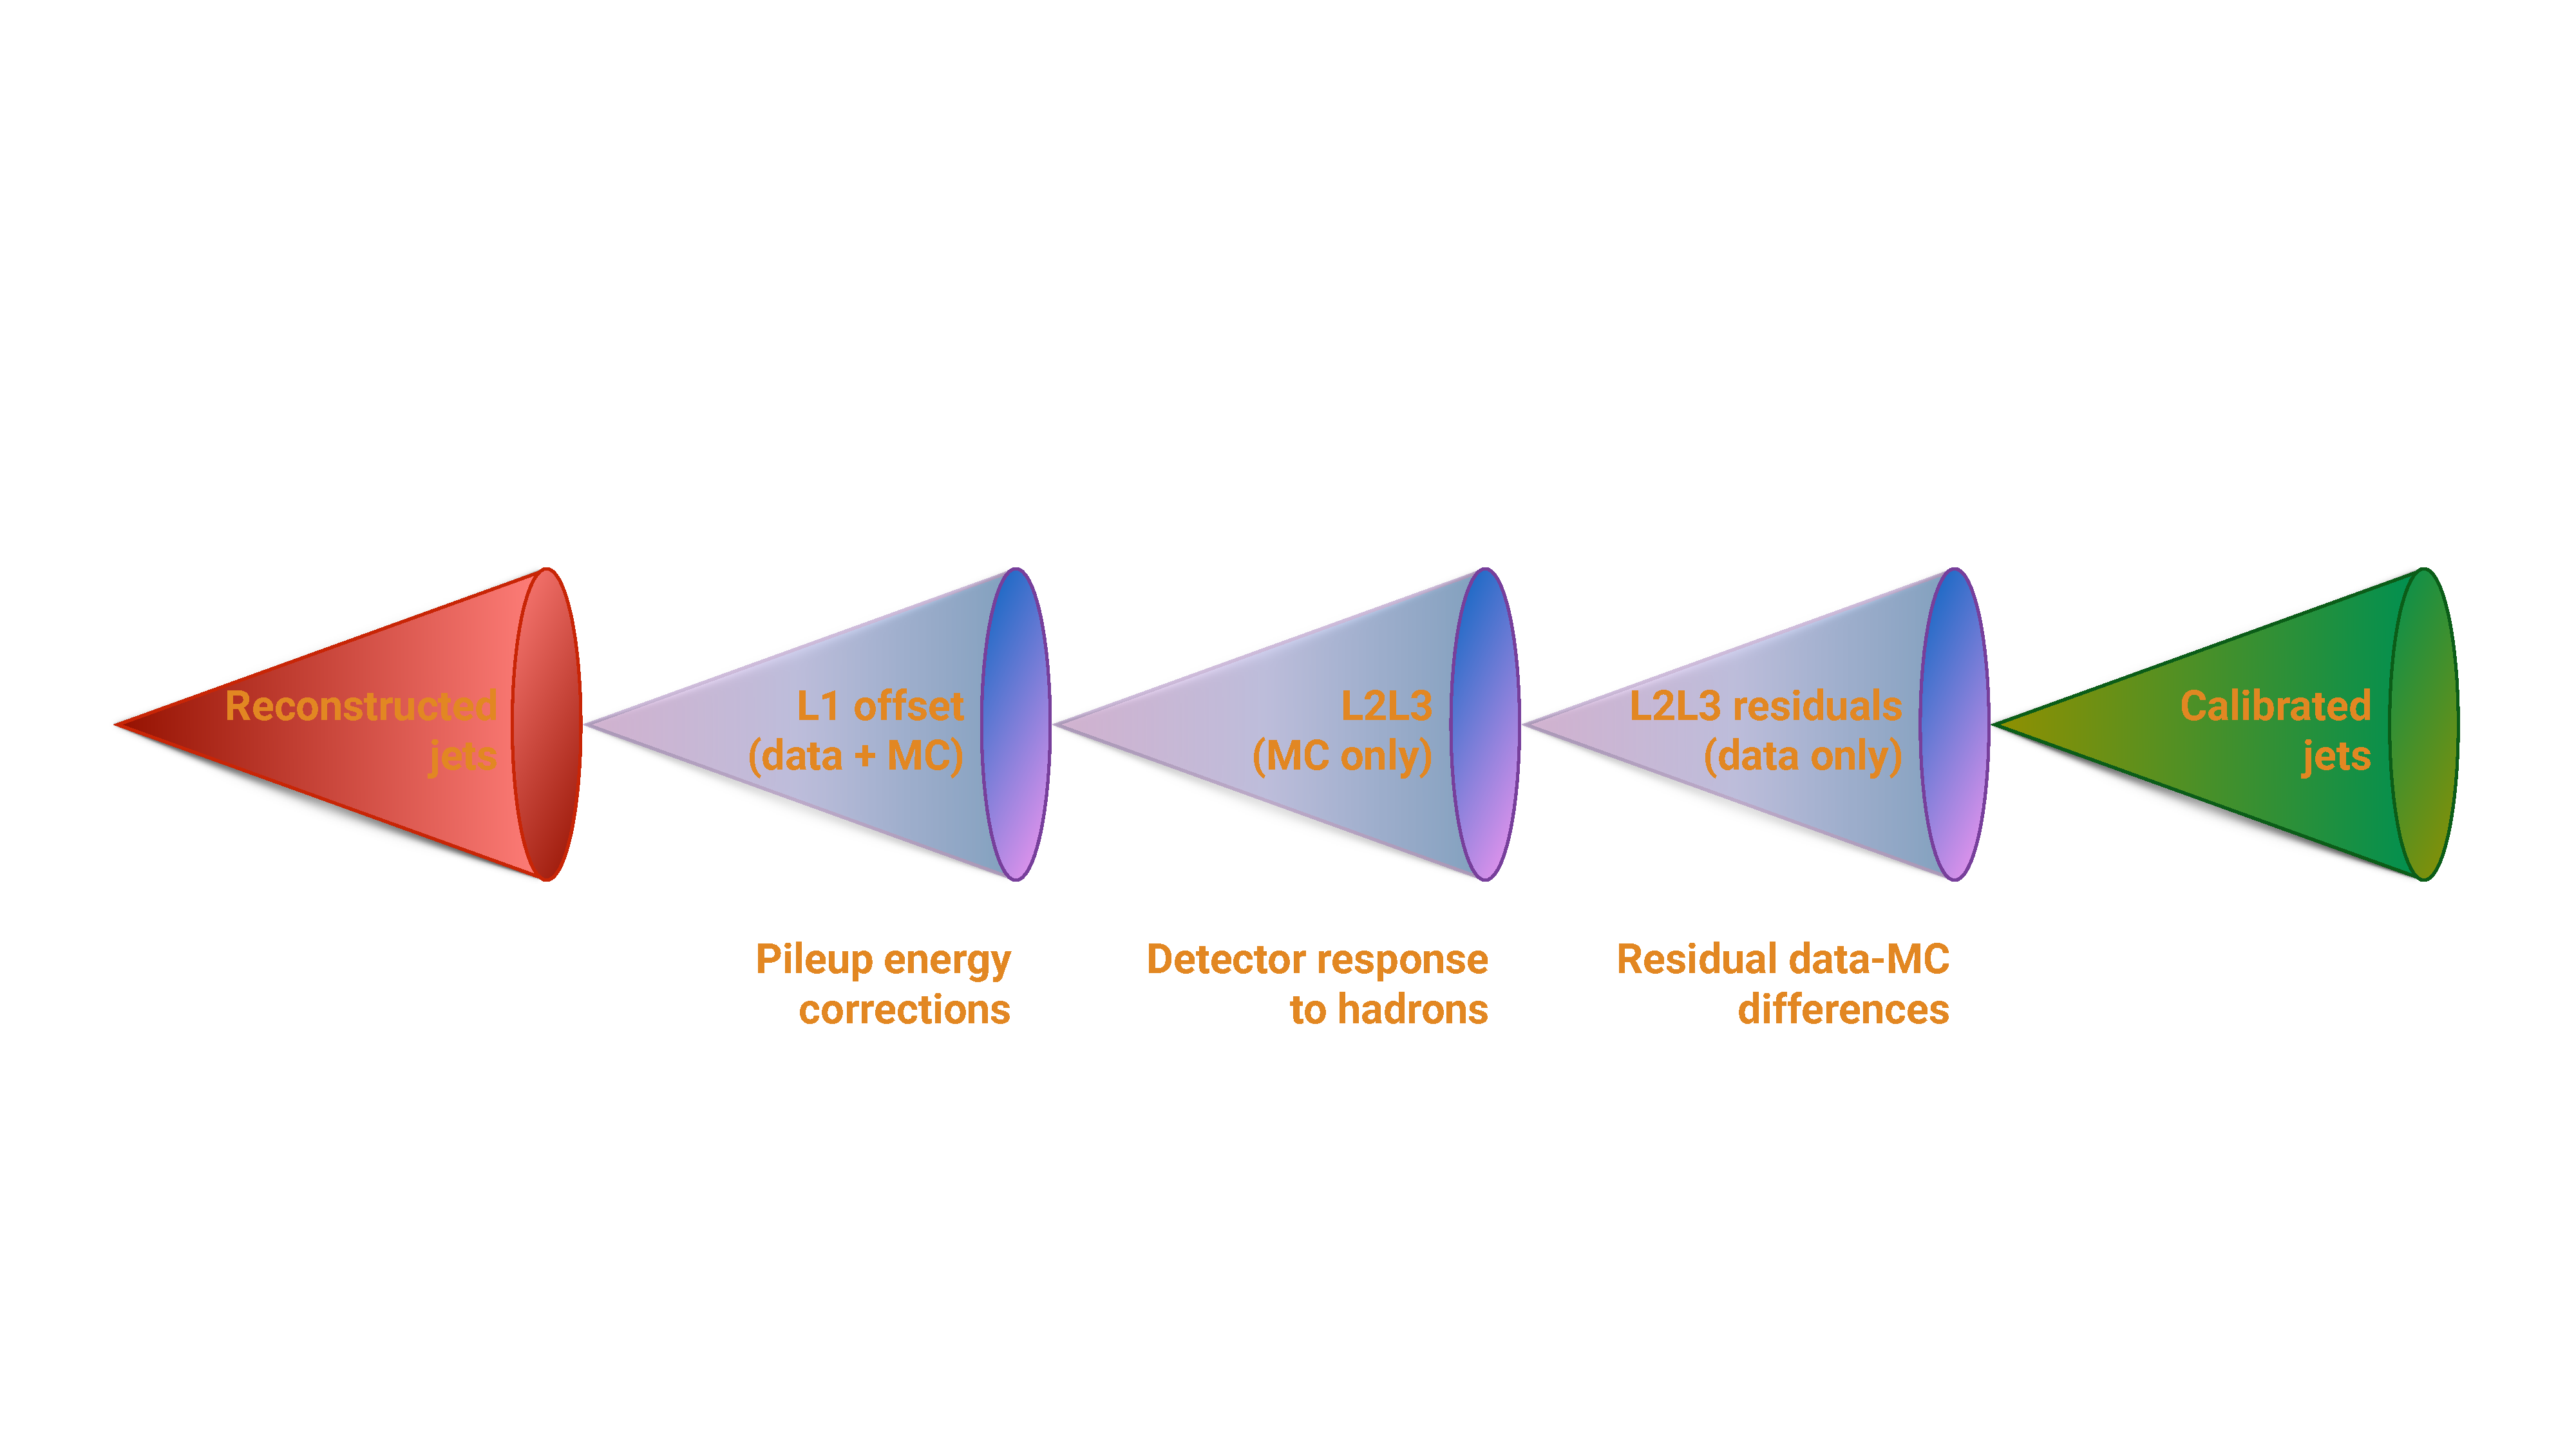
\includegraphics[width=0.99\textwidth]{figures/event_reconstruction/JEC.pdf}
    \caption{The CMS jet energy corrections are derived in three steps: A correction due to offset energy coming from pileup, applied to data and MC, a correction due to the particle-level jet response, also applied to data and MC and finally a correction to account for residual differences between data and MC.}
    \label{fig:objreco:jec}
\end{figure}

\subsubsection{L1 offset correction}
The largest correction is the L1 pileup offset correction, which is meant to subtract the additional energy in a jet due to pileup. This is done on an event-by-event basis through the \textit{jet area method} which uses the effective area of the jet multiplied by the average event energy density to calculate the size of the offset energy to be subtracted from each jet. An additional \PT- and $\eta$-dependent term is added in order to account for different pileup densities in different parts of the detector and for different jet energies. For data, an additional scalefactor to account for data and simulation differences is computed. This is done by constructing a \textit{Random Cone (RC)} centered at a given $\eta,\phi$ and dividing the energy density within that cone in data, evaluated in a dataset with no hard interactions (\textit{Zero Bias}), by that of the true energy offset in simulation

\subsubsection{L2 relative and L3 absolute corrections}
After L1 corrections are applied, corrections to account for the detector response to hadrons are derived based on the true detector response in QCD MC. The simulated particle response is defined as the ratio
\begin{equation}
  \textrm{R}_{\textrm{particle}}=\frac{p_{\textrm{T,reco}}}{p_{\textrm{T,particle}}}.
  \end{equation}
 These are derived in bins of particle-level \PT and reconstructed $\eta$: The L2 relative corrections are intended to make the detector response uniform and are derived as a function of $\eta$, while the L3 absolute corrections are derived as a function of jet \PT. These corrections are applied both to data and to MC.
 
\subsubsection{Residual data corrections}

After L1, L2, and L3 corrections are applied, two additional corrections are derived only for data in order to account for any residual discrepancies between data and MC. This is done by looking at the transverse momentum balance between a jet which is to be calibrated, and some reference object (either another jet, a Z boson, or a photon). If the jet energy scale is not equal to one, a \PT imbalance will be visible. The measurements are performed in a data sample of dijets, where the statistical uncertainty is small but the energy of the reference object poorly measured, as well as in $\PZ(\mu\mu)$+jet, $\PZ(ee)$+jet and $\gamma$+jet samples, where the energy of the \PZ and $\gamma$ is very well known but the statistics are small. \newline
The  "L2 relative" residual correction is measured in dijet events by comparing the measured \PT of the reference jet, required to be central with $\eta<1.3$, to that of the calibration jet, with an unconstrained $\eta$. This is done as a function of jet $\eta$, in bins of average jet \PT.
The "L3 relative" residual correction, is instead measured in $\PW/\gamma+\textrm{jet}$ events by comparing the measured jet \PT to the \PT of the precisely measured $\PZ/\gamma$, as a function of jet \PT.
The response, 
\begin{equation*}
R_{\textrm{jet,\PT}}=\frac{p_{T,\textrm{jet}}}{p_{T,\textrm{ref}}}
\end{equation*}
is then evaluated in data and in simulation. The ratio of the two, $R_{\textrm{data}}/R_{\textrm{MC}}$, defines the residual corrections.\newline\newline

The above description of jet energy corrections in CMS is meant as a rough, instructive summary only. A full description of the measurement techniques used in CMS can be found in~\cite{jme_jinst}. 

\section{Jet substructure reconstruction}
\label{sec:objreco:substructure}
In analyses looking for highly energetic ("boosted") vector bosons, the opening angle between the vector boson quark decay products becomes so small that the highly boosted boson appears as a single large jet instead of two well-separated smaller jets. The distance between the two quarks, in the case of a hadronic decay, depends on the mass of the vector boson and its \PT and goes as
\begin{equation}  
\Delta R = \frac{2 M_{V}}{p_{T,V}}.  
\end{equation}
Above a W boson \PT of 200 GeV, the two quarks are therefore merged into a single large cone jet of size R = 0.8. A sketch of the two different situation is shown in Figure~\ref{fig:objreco:mergedvsunmerged}. If the W \PT is well below 200 GeV, its decay products are two well-defined jets (left). However, once the W boson transverse momenta is approximately 200 \GeV, both the quarks are completely contained within a single jet (right), referred to as a W jet.
\begin{figure}[h] 
    \centering
    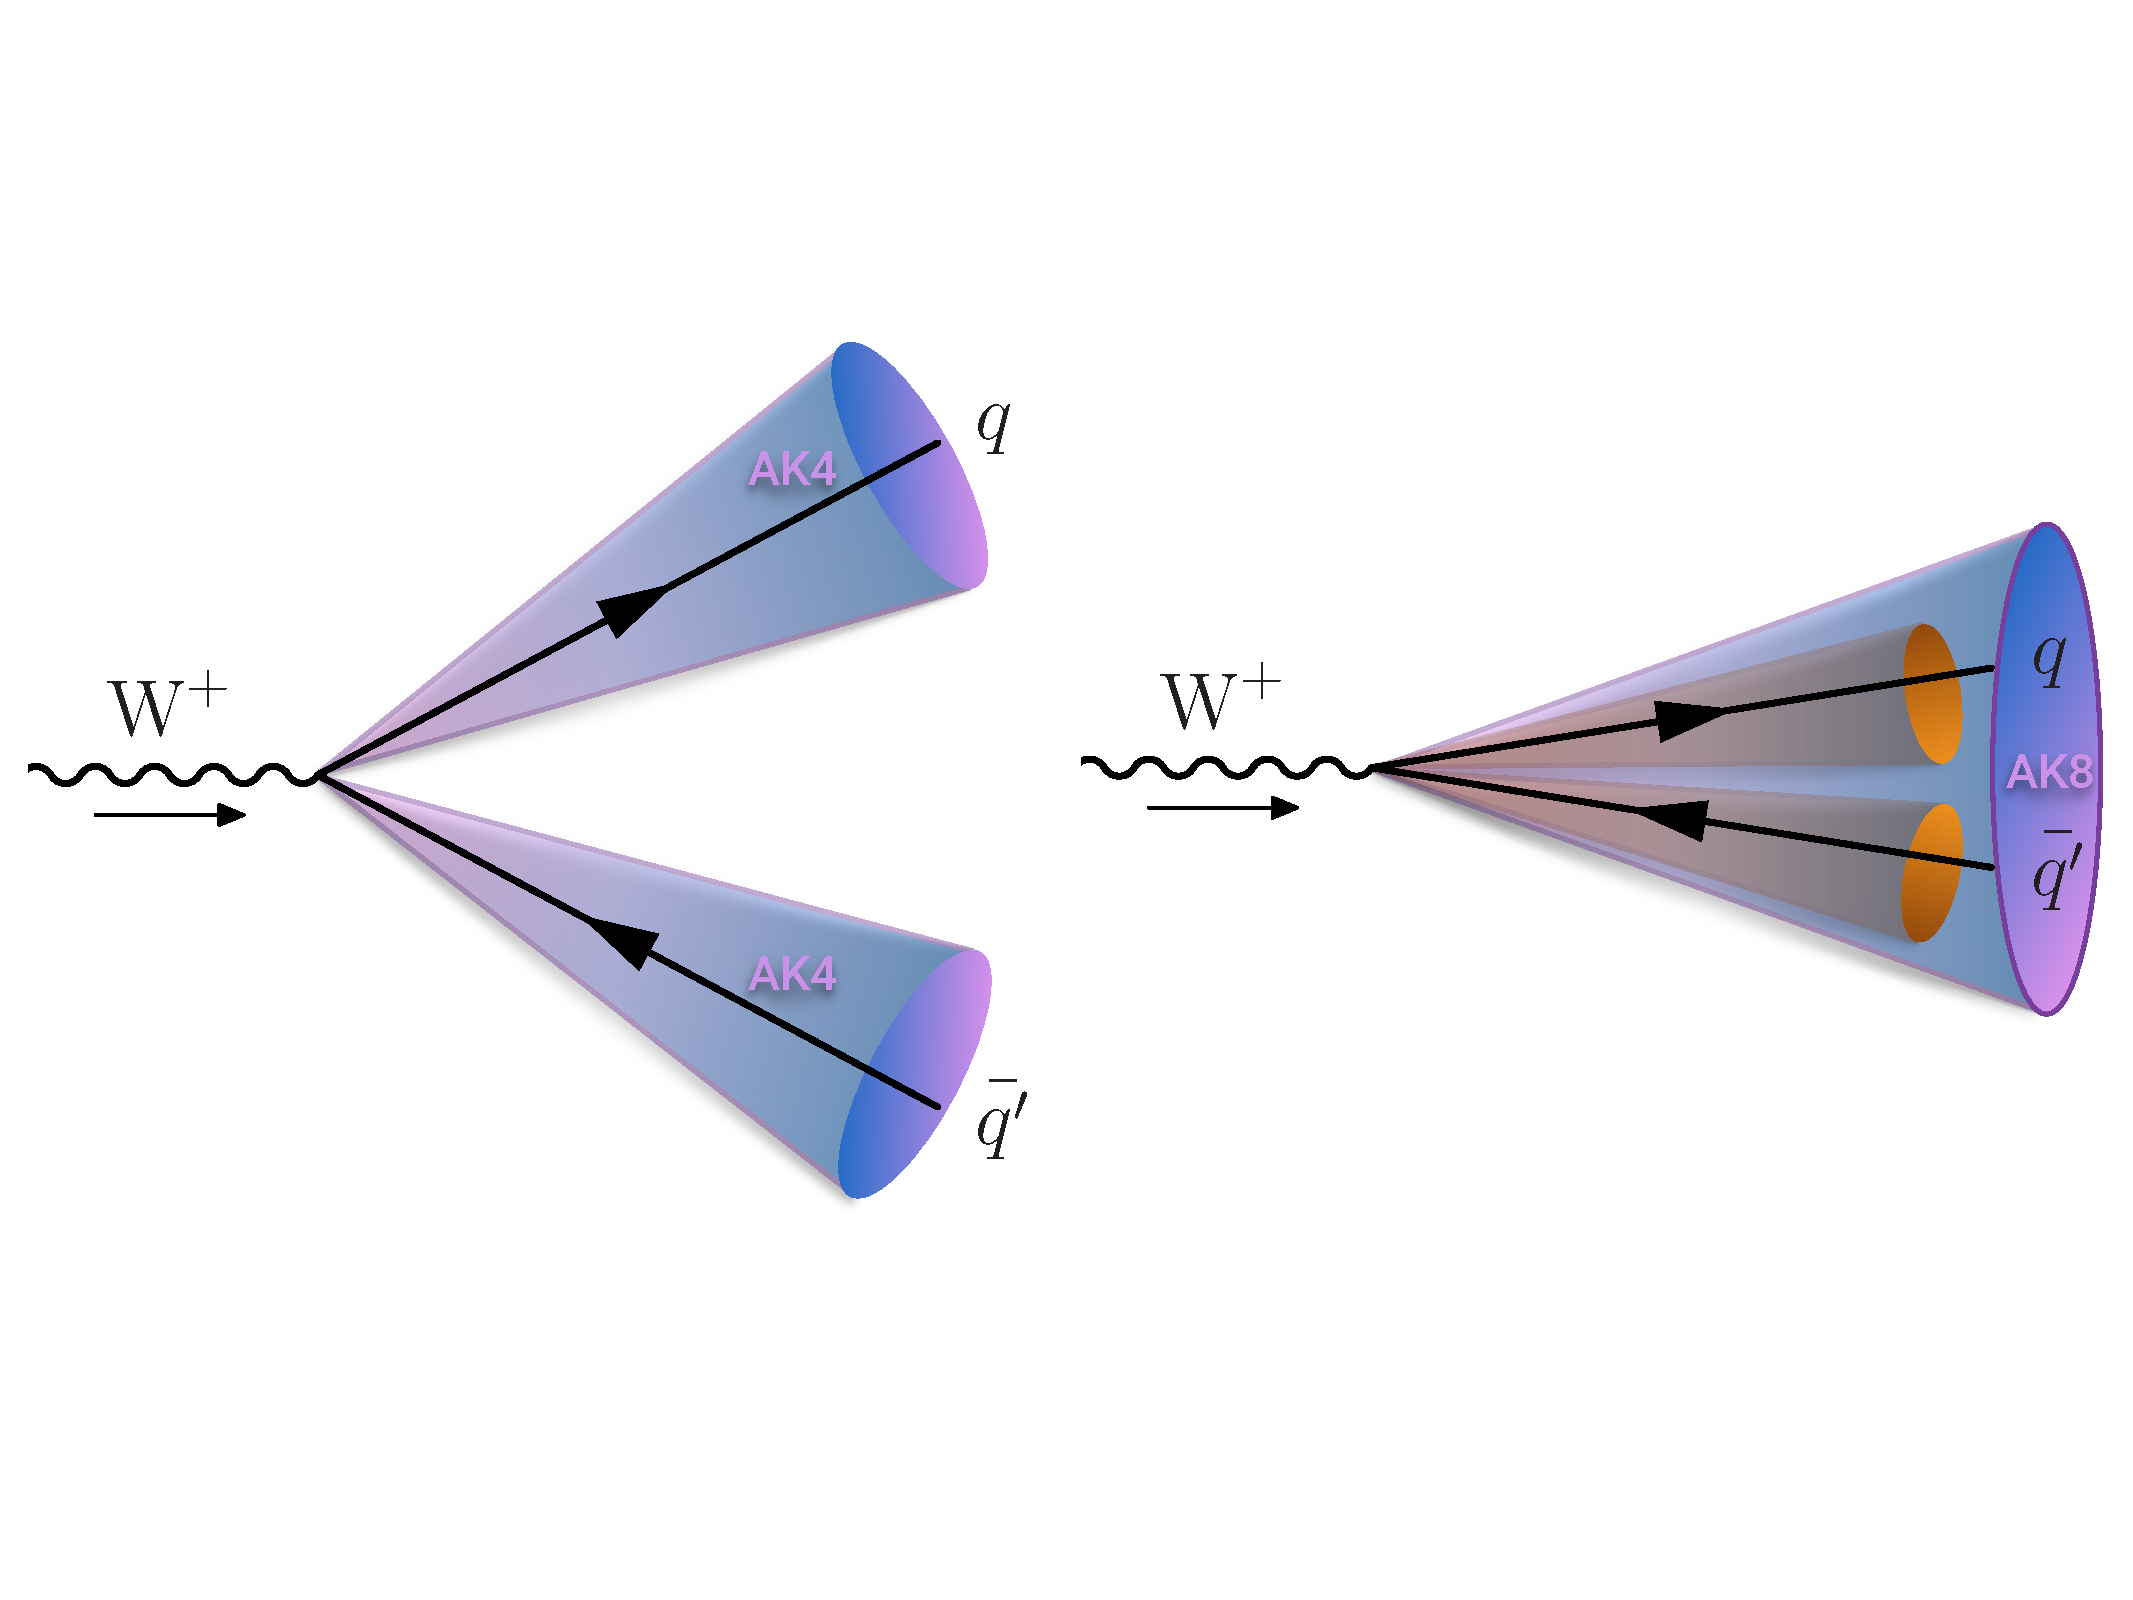
\includegraphics[width=0.70\textwidth]{figures/event_reconstruction/merged_vs_unmerged.pdf}
    \caption{If the mass of the resonance is low enough, the quark decay products of each vector boson are well separated and clustered into distinguishable AK4 jets (left). If the transverse momentum of the vector boson is greater than 200 GeV, the vector boson decay products are merged into one single large cone AK8 jet.}
    \label{fig:objreco:mergedvsunmerged}
\end{figure}
In order to distinguish jets from hadronically decaying vector bosons, either W or Z bosons, from those of quarks or gluons produced by QCD, the jet mass would in principle be a good discriminant since we know the W boson has a mass of around 80 GeV while the quark or gluon mass is close to zero. At very high transverse momenta, however, the width (and therefore the mass) of QCD jets may become equally large. In addition, diffuse radiation caused by the underlying event and pileup give rise to a significant number of additional particles in the event contributing to the total jet mass.
Therefore, being able to accurately and efficiently separate highly boosted QCD jets from highly boosted vector bosons requires other methods. In order to remove the underlying event and pileup, algorithms like PUPPI and CHS can be used. In order to improve the mass resolution further, dedicated grooming algorithms must be applied.

\subsection{Grooming}
\label{sec:objreco:grooming}
Grooming was introduced as a tool to improve the mass resolution of large radius jets without significantly changing the background and signal event numbers. It consists of removing the softest parts of a jet in order to resolve its "true" mass, by means of reclustering and identifying soft particles within the jet that can be removed.

\subsubsection{Trimming}
\label{sec:objreco:trimming}
The trimming algorithm~\cite{Krohn:2009th} is a grooming algorithm mostly used at trigger level in CMS (also where it is used in this thesis) due to it being less aggressive than other grooming algorithms. It works in the following way: starting from a large jet clustered with either anti-\kt or C/A (in the case of CMS), it reclusters the jet using the \kt algorithm in order to create subjets of some size $R_{sub}$.  It then proceeds to check whether each subjet has a momentum fraction above a certain threshold,
\begin{equation*}
p_{T,i}/p_{T,jet}>p_{T,frac}.
\end{equation*}
If the subjet fails this requirement, it is removed. The remaining subjets are then assembled into a new "trimmed" jet.
The effect of trimming on real W boson jets and QCD quark or gluon jets for different values of $r_{sub}$ and $p_{T,frac}$ is shown in Figure~\ref{fig:objreco:trimming}. 
The best signal mass resolution is obtained with $r_{sub}=0.2$ and $p_{T,frac}=0.03$, which is also the parameter setting that provides the best signal discrimination from background by pushing the QCD jet mass closer to zero. These are the default values of the tuned parameters of the trimming algorithm in CMS ($r_{sub}=0.2$ and $p_{T,frac}=0.03$).
\begin{figure}[h] 
    \centering 
    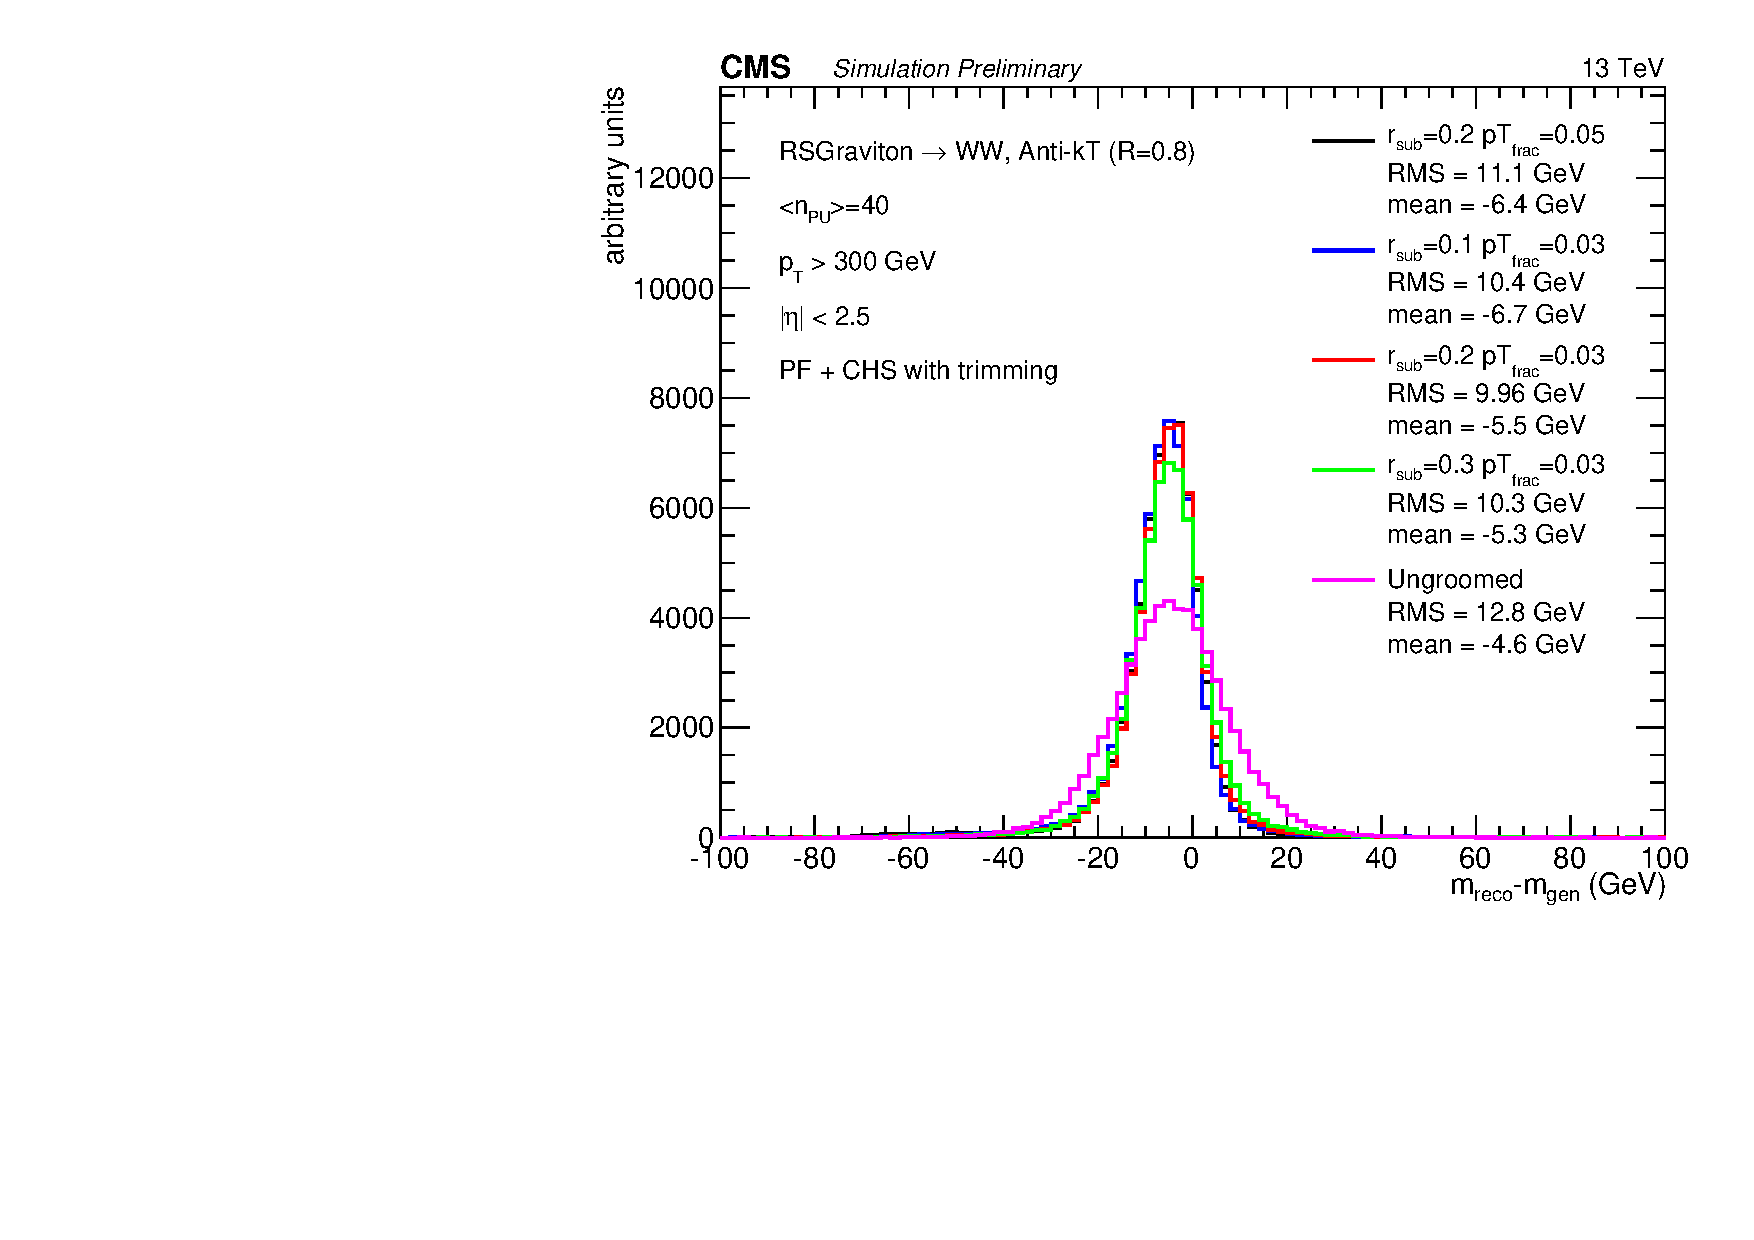
\includegraphics[height=6cm]{figures/event_reconstruction/sig_trimming.pdf}
    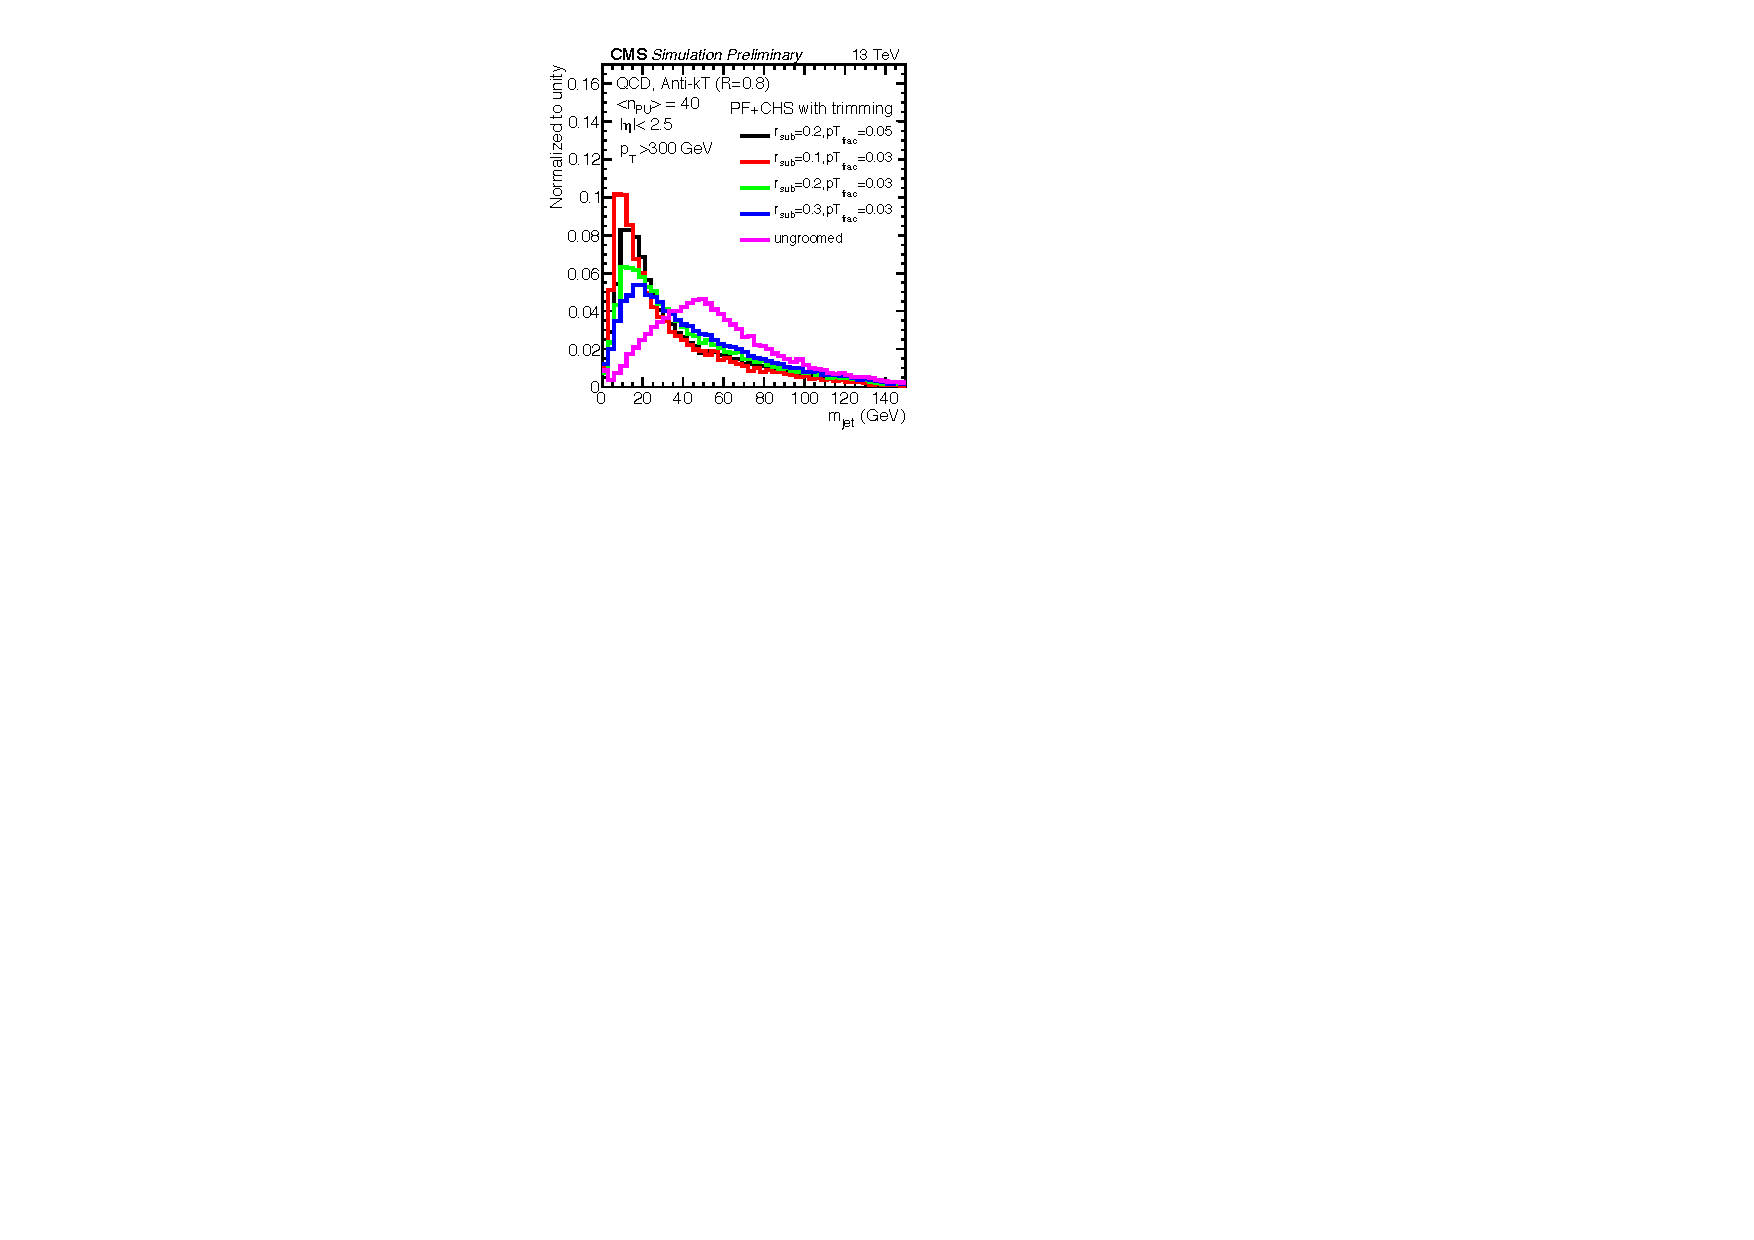
\includegraphics[height=6cm]{figures/event_reconstruction/bkg_trimming-noData.pdf}
    \caption{The effect of trimming on a signal jet (left) and a background jet (right) for different values of the tuned parameters $r_{sub}$ and $p_{T,frac}$~\cite{CMS-PAS-JME-14-001}.}
    \label{fig:objreco:trimming}
\end{figure}

\subsubsection{Pruning}
\label{sec:objreco:pruning}
The pruning algorithm, in addition to removing soft particles, has an additional requirement on the distance between any recombination that is at wide angle.
It proceeds by reclustering the jet with the C/A algorithm, requiring at each step that
\begin{equation*}
\frac{ \textrm{min}(p_{T,i},p_{T,j}) }{ p_{T,P} } > z_{cut} \quad \textrm{ and } \quad \Delta R_{i,j} < D_{cut} = \frac{2 r_{cut} m_{jet}}{\PT}.
\end{equation*}
The first requirement is a requirement on the hardness of the combination. The variables $p_{T,i}$ and $p_{T,j}$ correspond to the transverse momenta of each protojet (single particle or group of particles already combined in a previous step) and $p_{T,P}$ is the combined \PT of the two. The protojet with the lowest transverse momenta is removed if its hardness is below $z_{cut}$, or if it forms an angle wider than $D_{cut}$ relative to the axis of the recombination of the two protojets. In CMS, the tuned parameters are set to $r_{cut}=0.5$ and where $z_{cut}=0.1$. Figure~\ref{fig:objreco:pruning} shows the ungroomed as well as the pruned jet mass distribution for signal (left) and background (right) jets. The highest amount of signal and background separation in CMS, is achieved with $r_{cut}=0.5$ and $z_{cut}=0.1$.
\begin{figure}[h] 
    \centering
    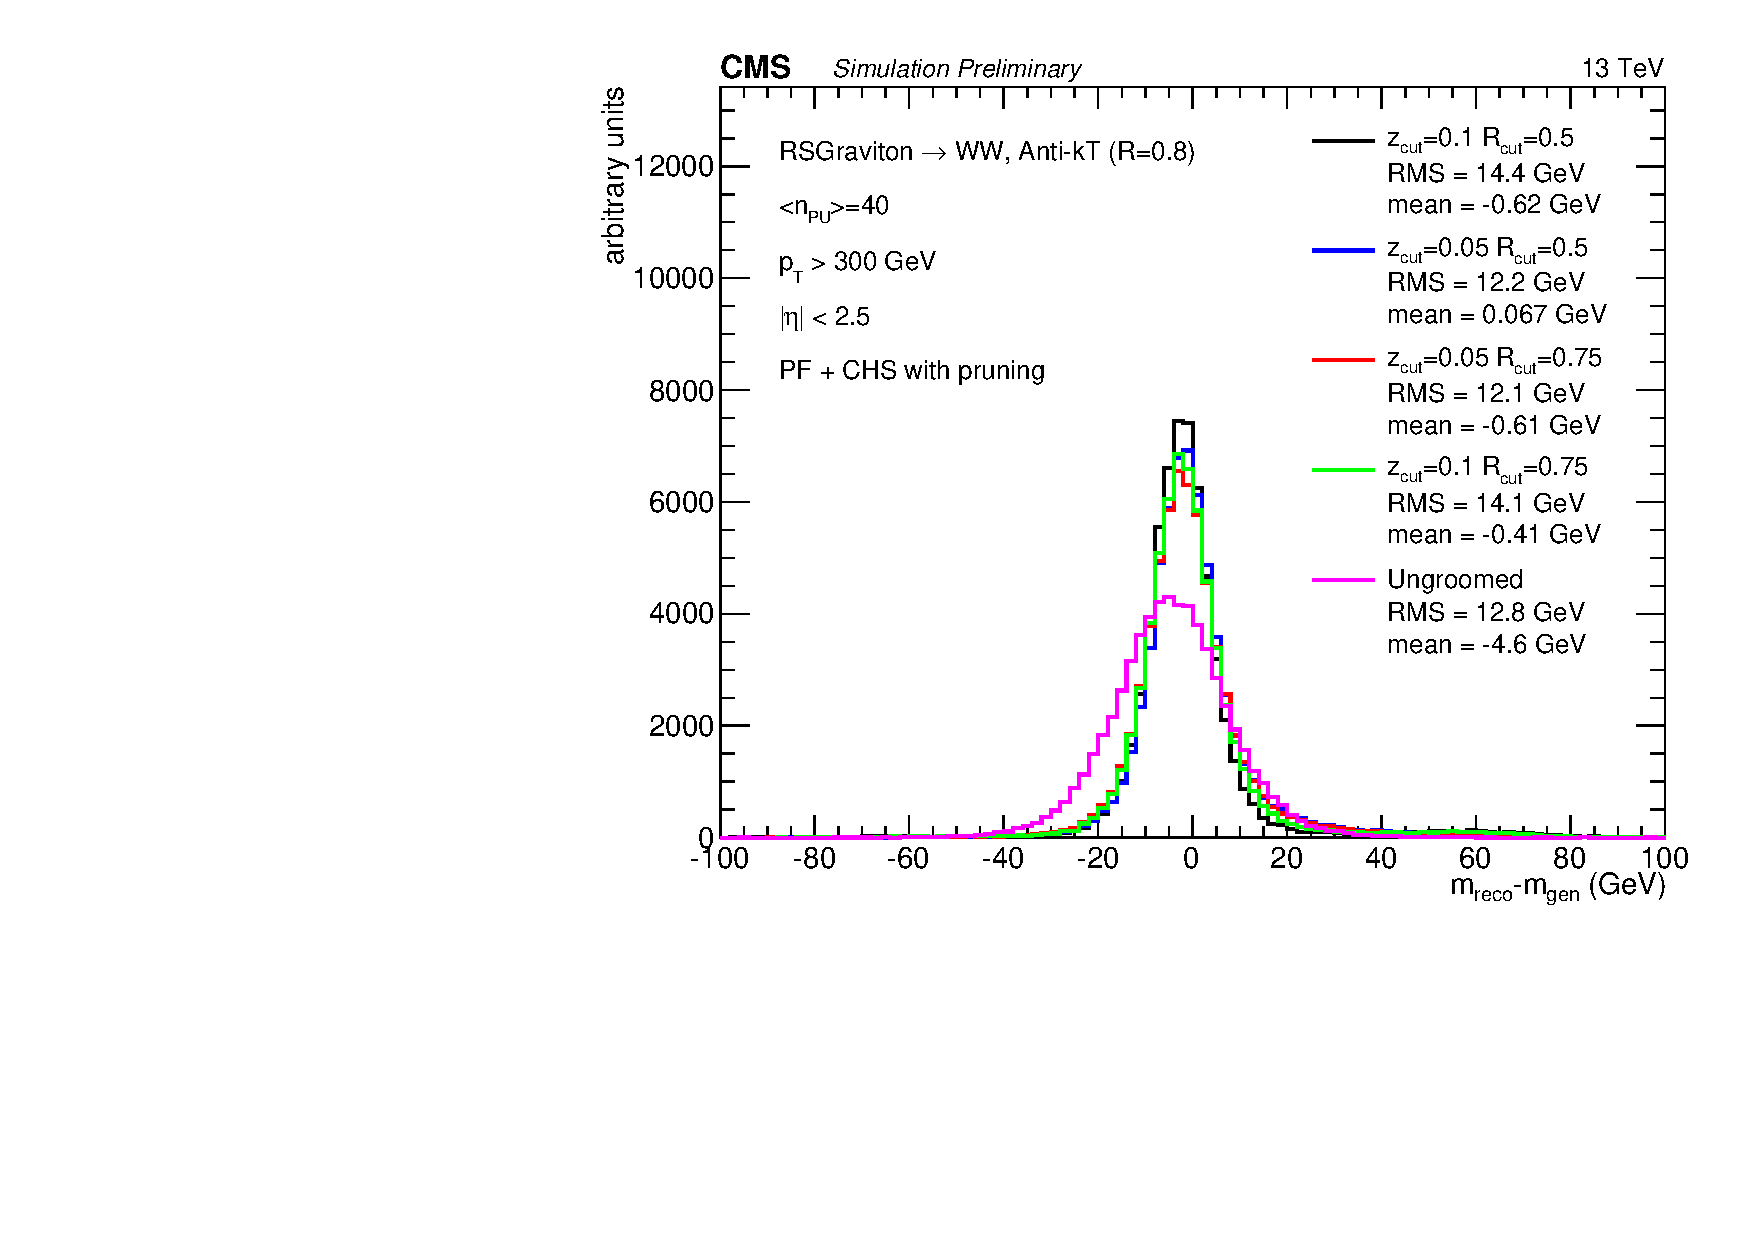
\includegraphics[height=6cm]{figures/event_reconstruction/sig_pruning.pdf}
    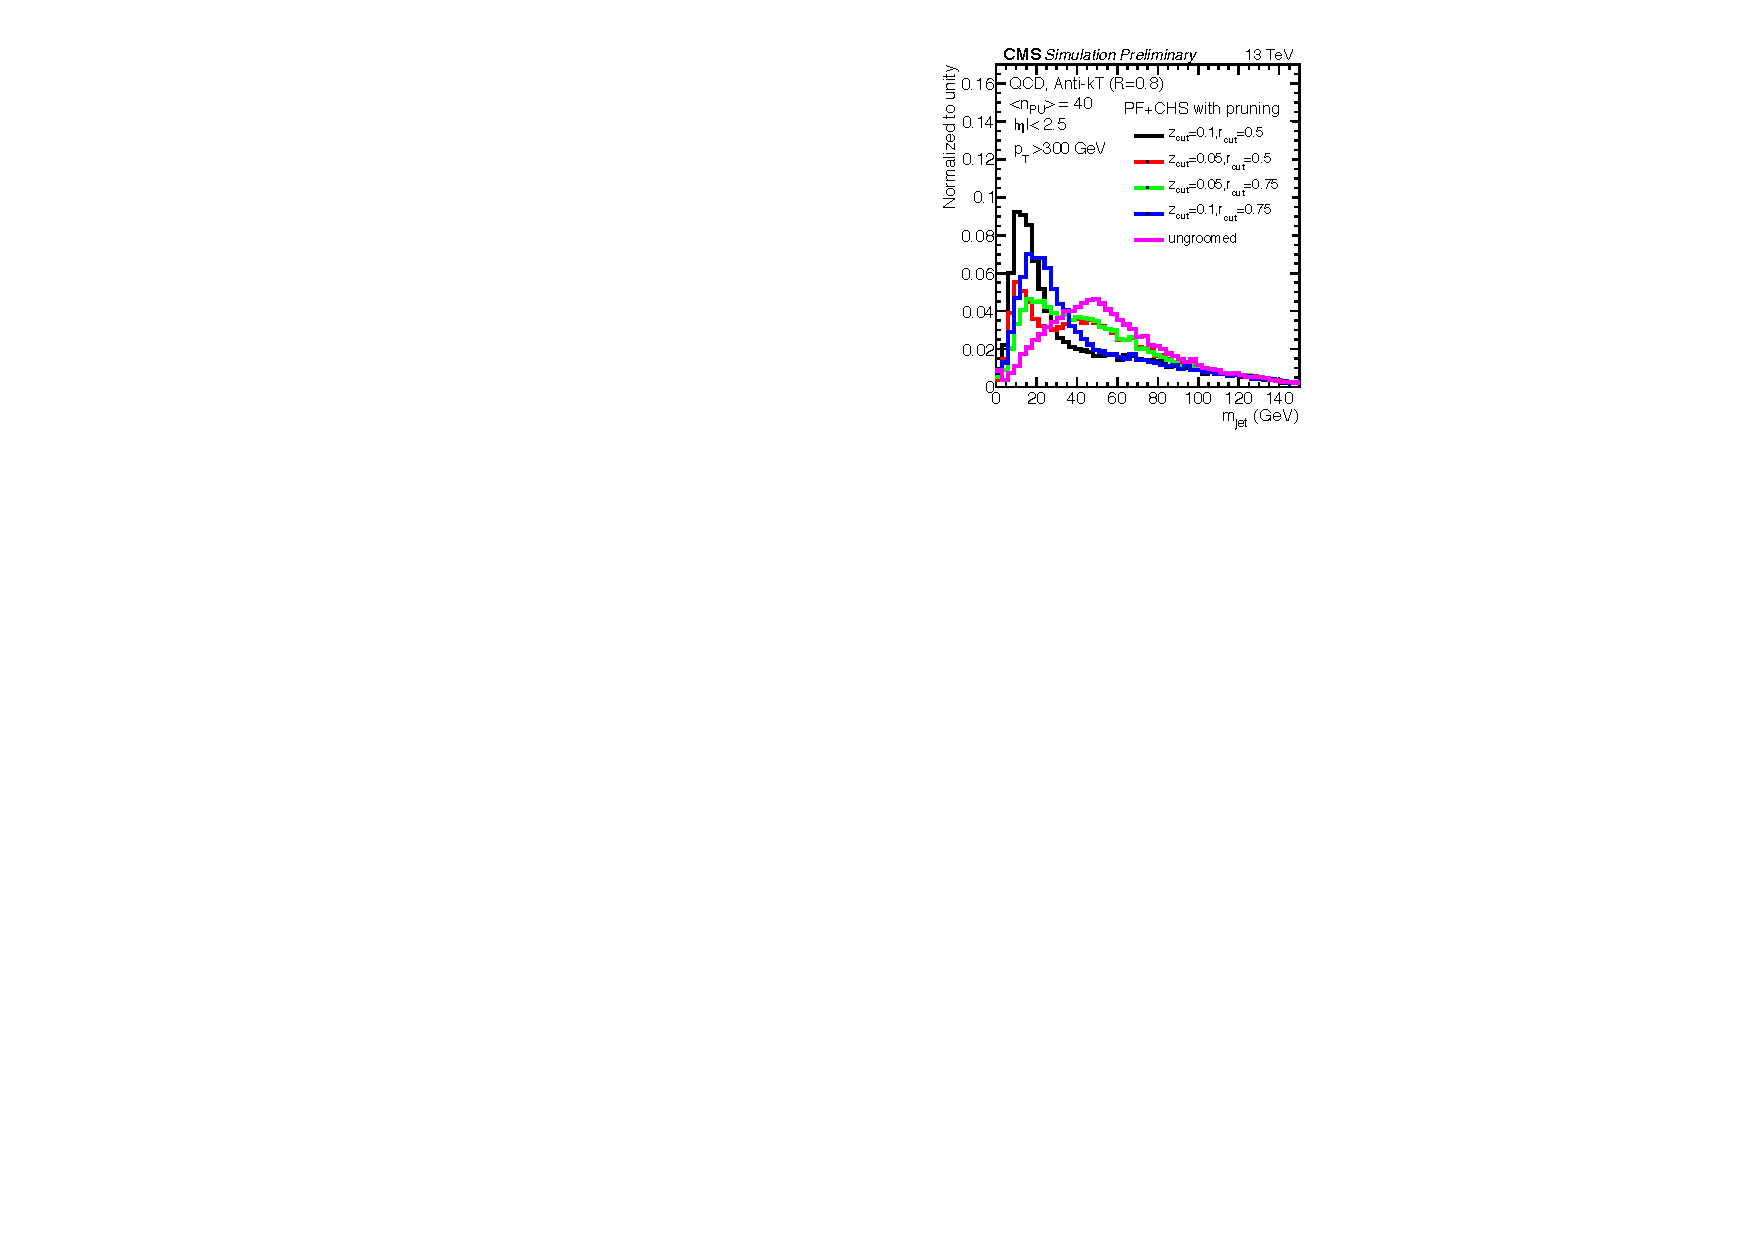
\includegraphics[height=6cm]{figures/event_reconstruction/bkg_pruning-noData.pdf}
    \caption{The effect of pruning on a signal jet (left) and a background jet (right) for different values of the tuned parameters $z_{cut}$ and $r_{cut}$~\cite{CMS-PAS-JME-14-001}.}
    \label{fig:objreco:pruning}
\end{figure}



\subsubsection{Modified Mass Drop Tagger and Soft Drop}
\label{sec:objreco:softdrop}
The modified mass drop tagger (mMDT)~\cite{Dasgupta:2013ihk} (a modified version of the originally suggested mass drop tagger ~\cite{Butterworth:2008iy}) is based on the idea that a \PW or \PZ jet is formed by two quark subjets and that, therefore, the mass of each subjet is much smaller than their combined mass (and much smaller than the mass of the boson itself). A QCD jet is, on the other hand, formed by continuous soft radiation, meaning that its heaviest subjet should be close to the mass of the jet itself. The mMDT tagger therefore starts from an already clustered jet, reclusters it with the C/A algorithm and then declusters it again, defining subjets $s_1$ and $s_2$. It then looks for a significant mass drop going from the total jet mass to the mass of each subjet, and checks that the splitting is not too asymmetric. The modified mass drop condition is generalized through the soft drop declustering method~\cite{Larkoski:2014wba}, simply called Soft Drop, which allows for different types of angular requirements to enter the condition. The Soft Drop condition is the following,
\begin{equation*}
\frac{ \textrm{min}(p_{T,1},p_{T,2}) }{ p_{T,1}+p_{T,2} } > z_{cut} \frac{\Delta R_{12}}{R_0}^\beta.
\end{equation*}
If no significant mass drop occurred and the splitting is not too asymmetric, the condition is met and the full jet is deemed the softdrop jet. Otherwise only the highest-\PT subjet is kept and the declustering continues. If the jet can not be declustered any further, it can either be removed from consideration, so-called "tagging"-mode, or deemed the final soft-dropped jet, "grooming"-mode. A $\beta=0$ corresponds to the modified mass drop tagger and removes all soft emission from the jet. For $\beta>0$, soft radiation is removed, but some fraction of soft-collinear radiation is kept. Lastly, with $\beta<0$, Soft Drop can remove soft as well as collinear radiation.
The performance of Soft Drop on W jets and QCD quark/gluon jets for different values of $\beta$ is shown in Figure~\ref{fig:objreco:softdrop}. The modified mass drop tagger (Softdrop with $\beta$=0) with $z_{cut} = 0.1$ is the default Soft Drop settings in CMS, due to it providing the best signal/background discrimination while maintaining an excellent signal mass resolution. 
\begin{figure}[h!] 
    \centering 
    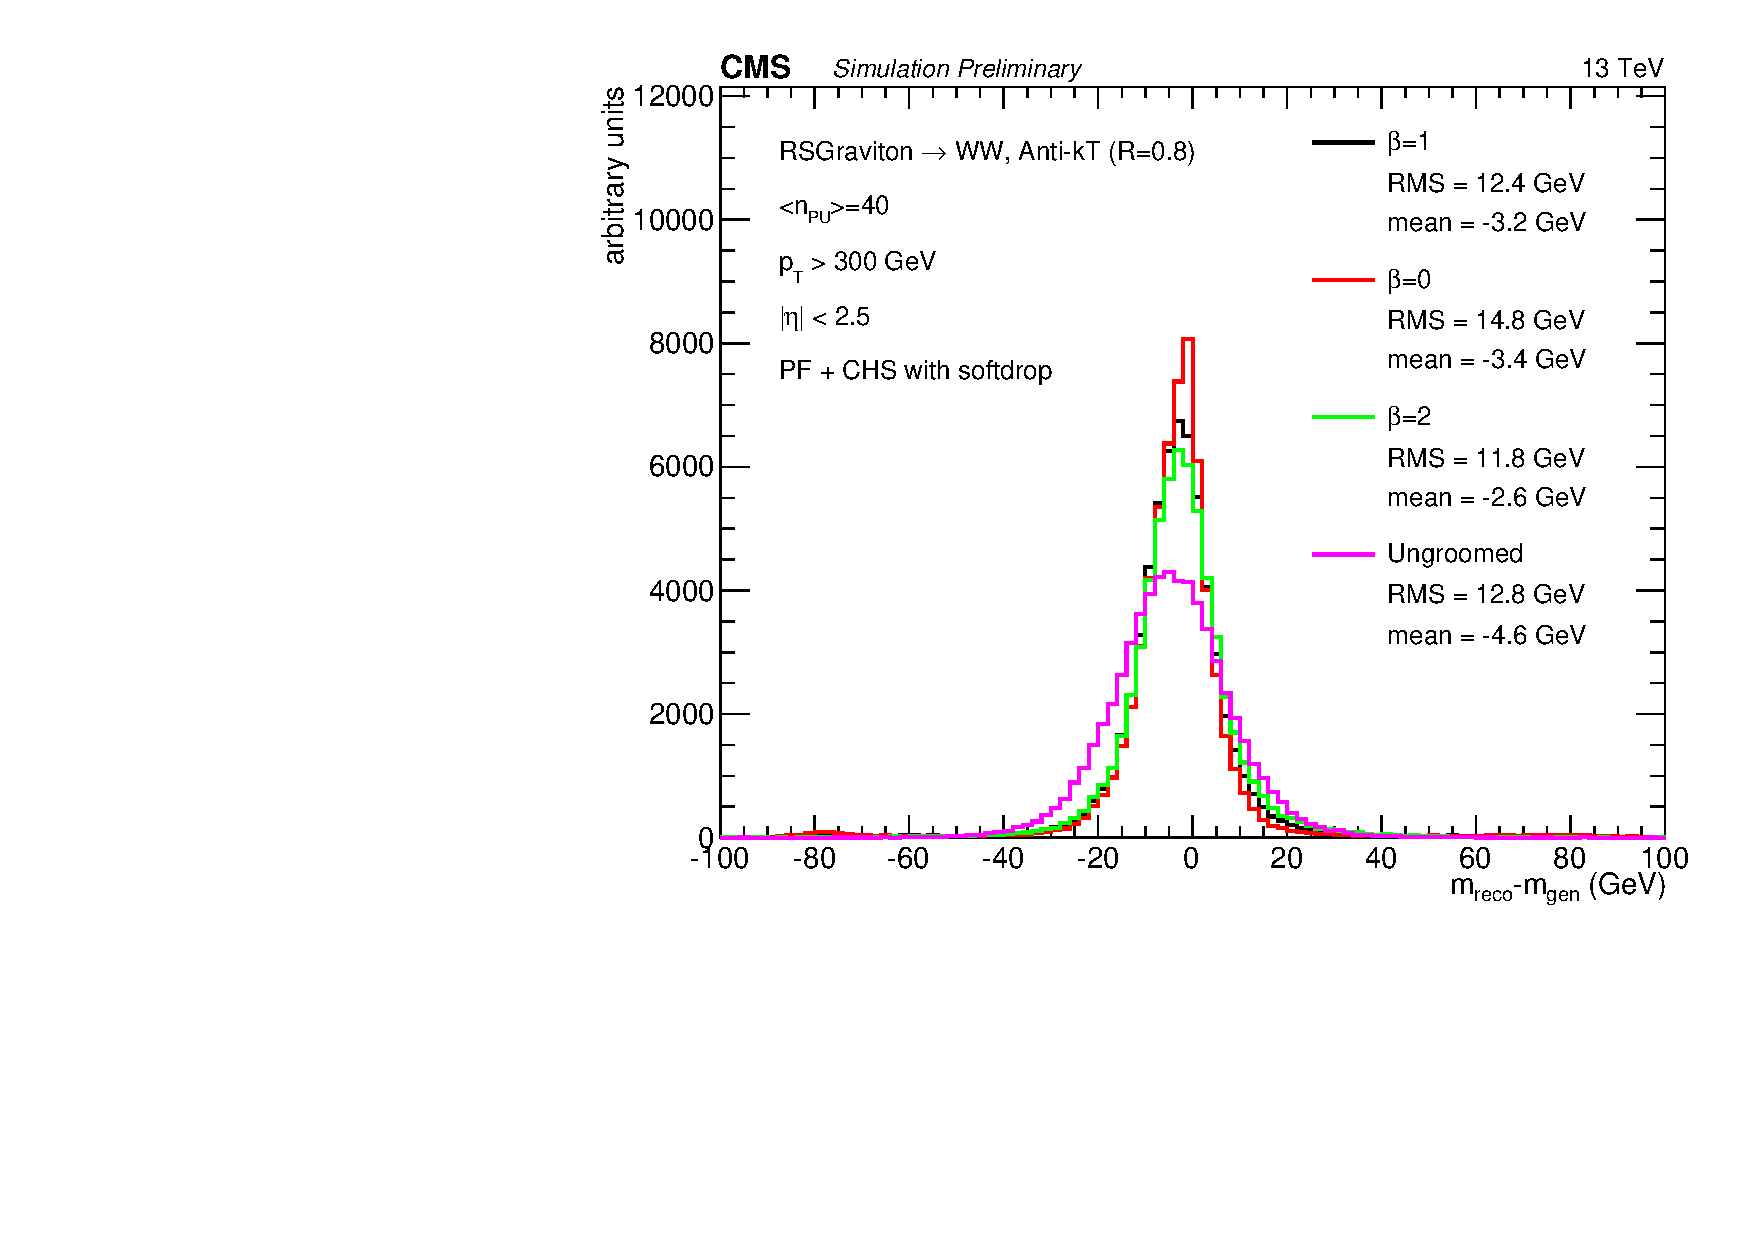
\includegraphics[height=6cm]{figures/event_reconstruction/sig_sd.pdf}
    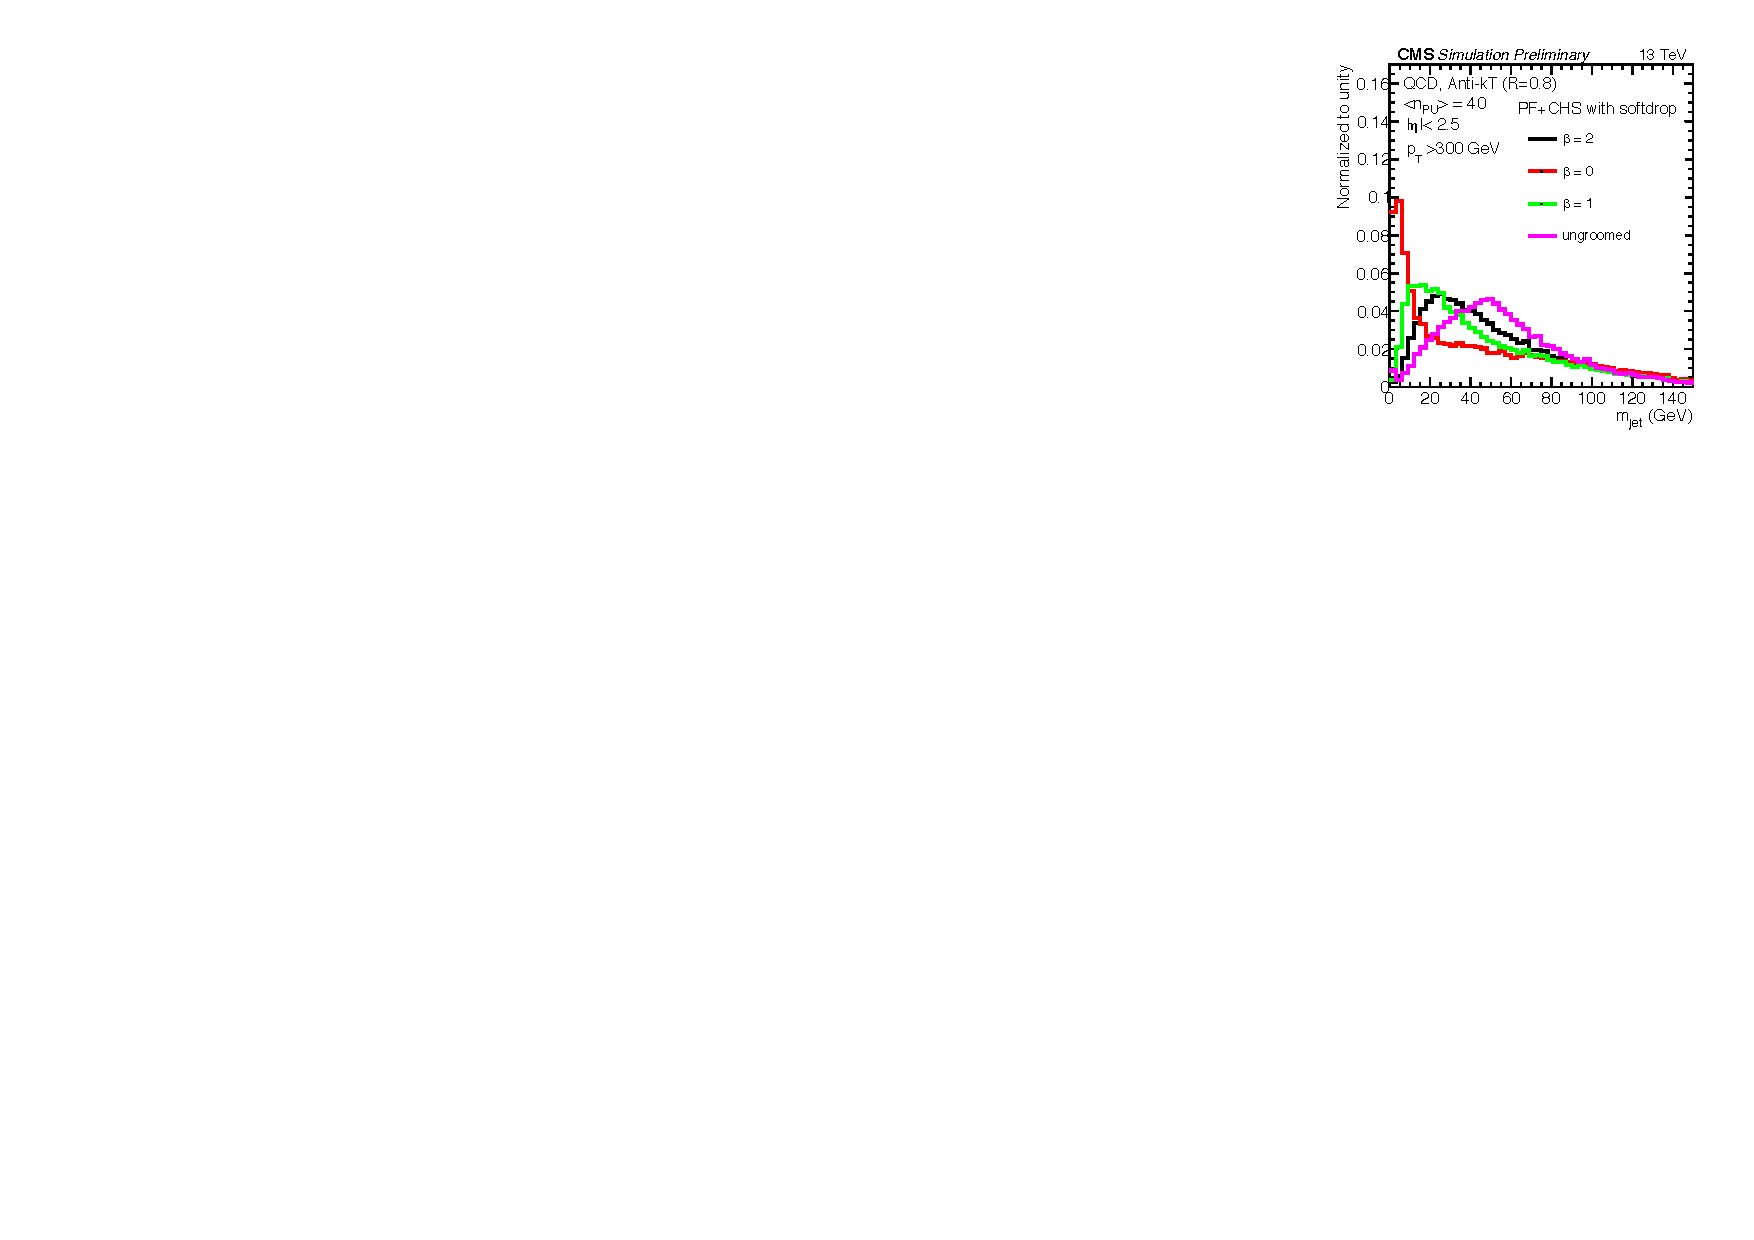
\includegraphics[height=6cm]{figures/event_reconstruction/bkg_softdrop-noData.pdf}
     \caption{The effect of softdrop on a signal jet (left) and a background jet (right) for different values of the tuned parameters $\beta$. $\beta=0$ corresponds to the Modified Mass Drop Tagger, which is the default Softdrop setting in CMS ~\cite{CMS-PAS-JME-14-001}.}
     \label{fig:objreco:softdrop}
 \end{figure}

\subsection{N-subjettiness}
\label{sec:objreco:nsubj}
After using the algorithms above, there is still information in the jet structure itself that can distinguish W/Z jets from quark/gluon jets. A \PW or \PZ jet consists of two well-defined high-\PT subjets. A quark/gluon jet instead is made from a single parton, and consists of several large angle, asymmetric splittings, as illustrated in Figure~\ref{fig:objreco:onevstwoprong}.
\begin{figure}[h!] 
    \centering 
    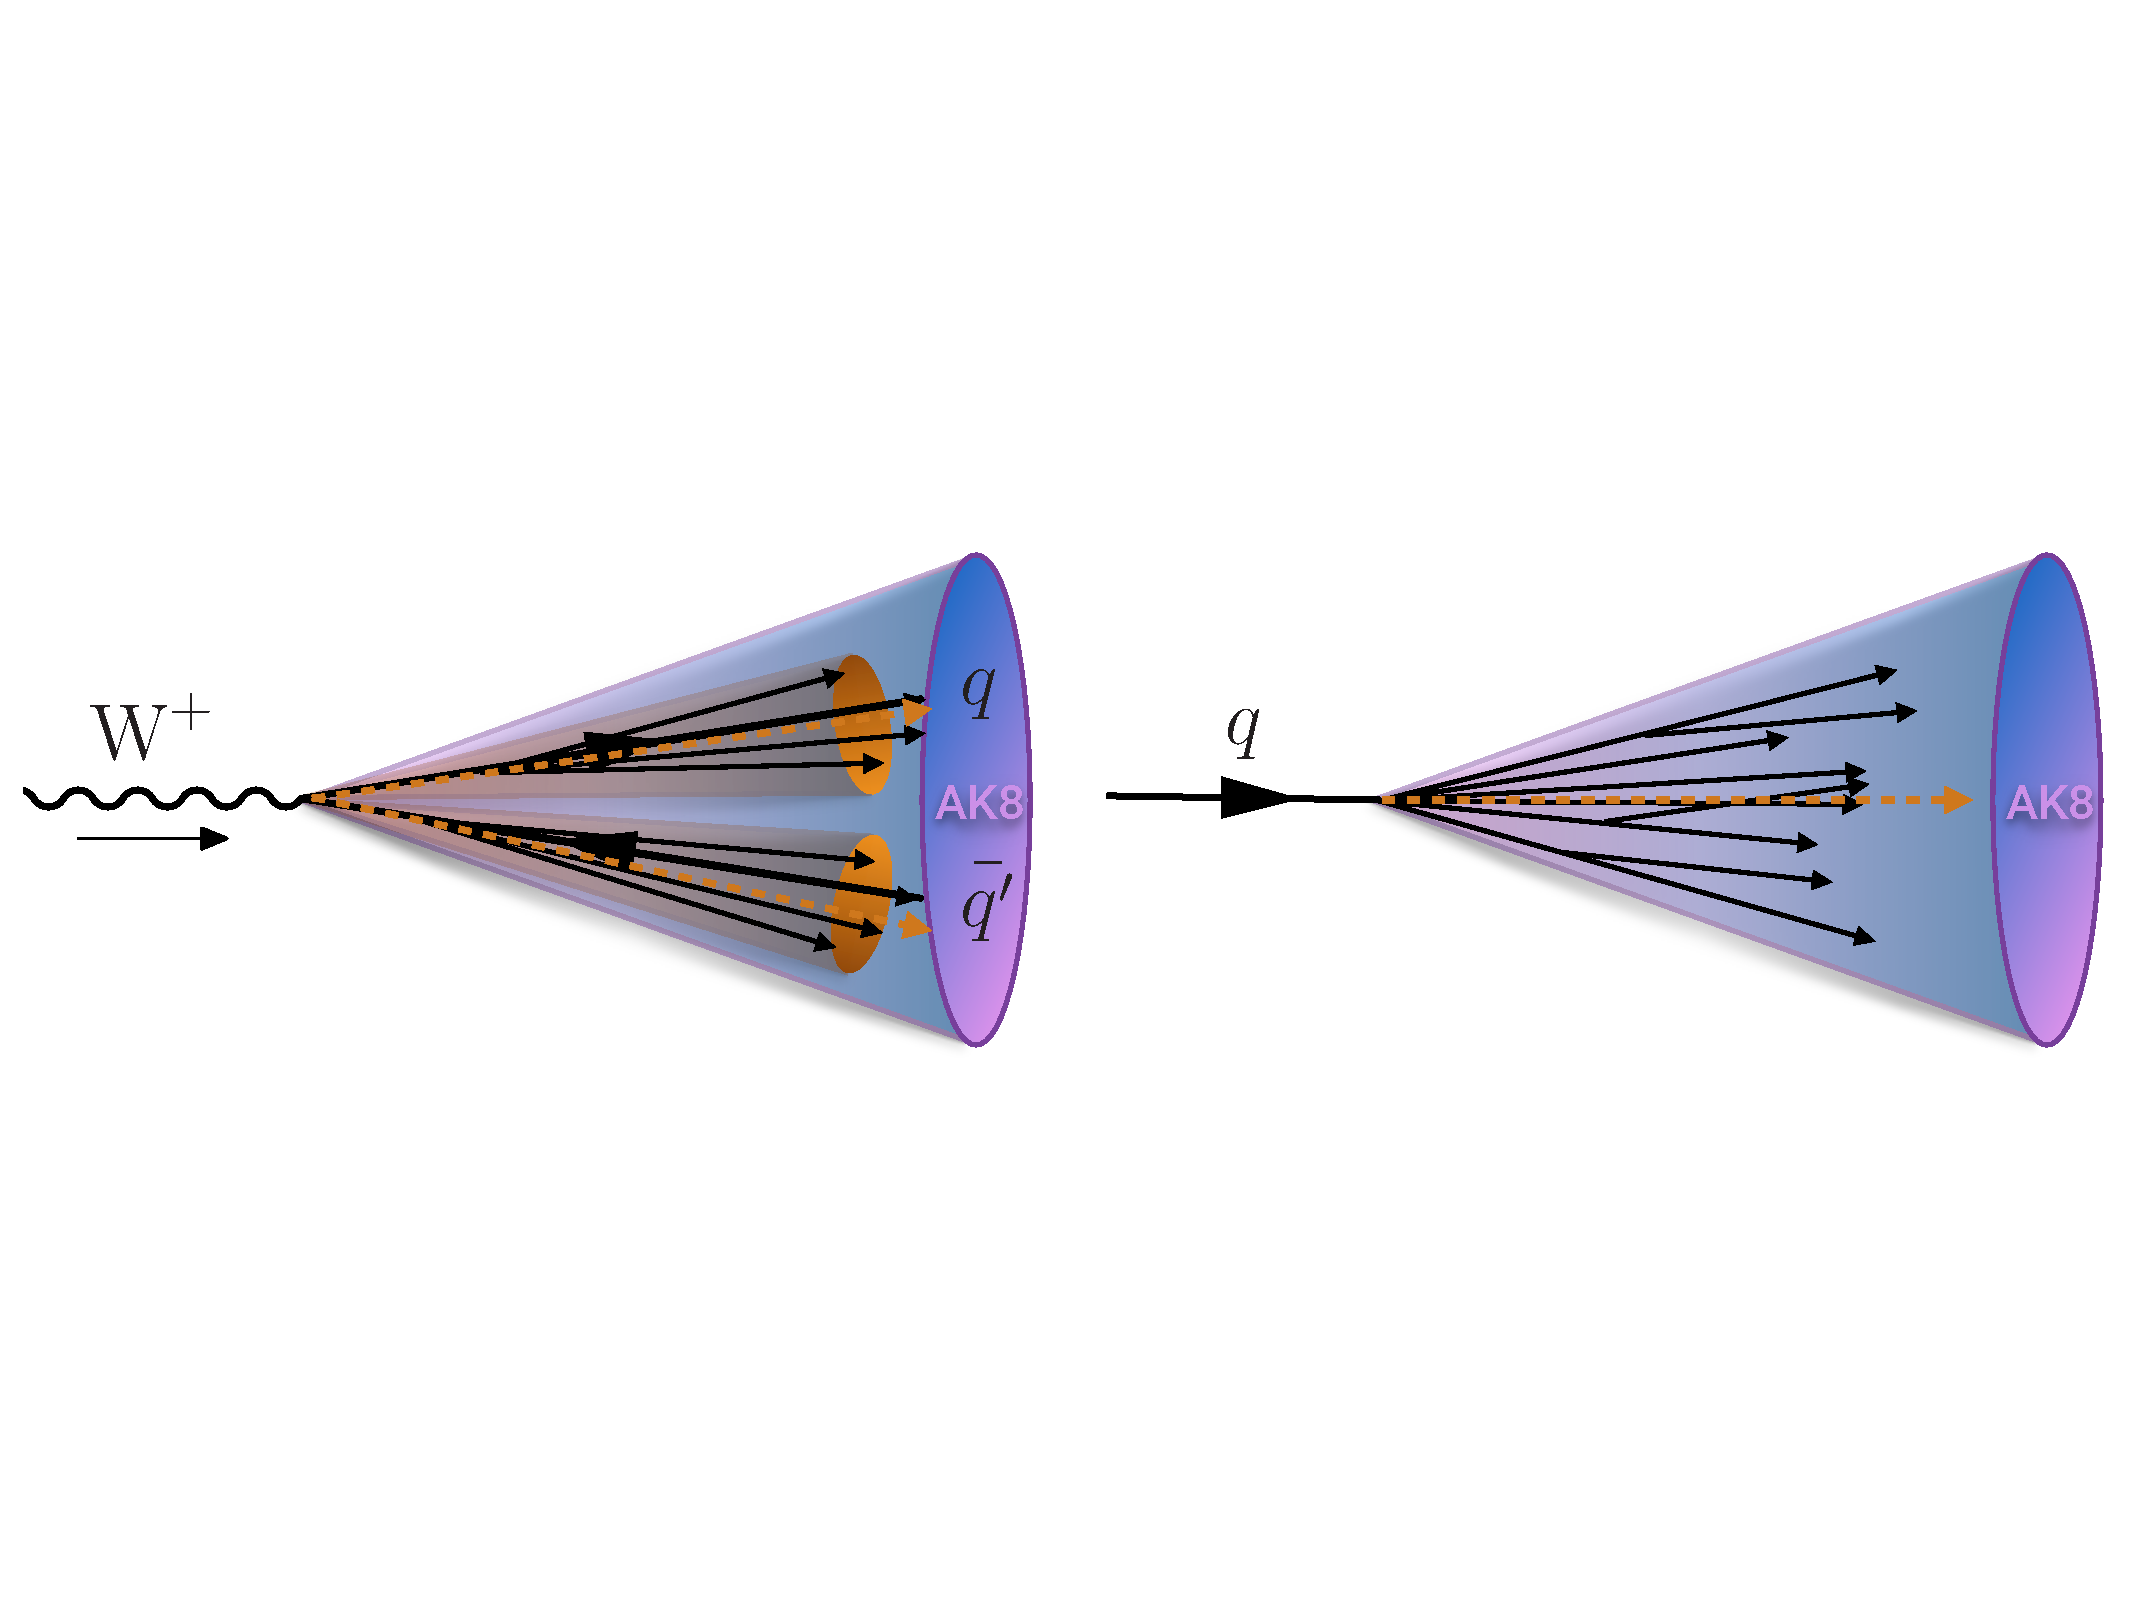
\includegraphics[width=0.790\textwidth]{figures/event_reconstruction/tau21_sketch.pdf}
     \caption{A jet stemming from the decay of a \PW will usually have two well-separated high-\pt subjets, while a jet with a single-prong origin consists of several large angel splittings.}
     \label{fig:objreco:onevstwoprong}
 \end{figure}
The N-subjettiness algorithm~\cite{Thaler:2010tr} takes advantage of this fact by attempting to count the number of hard sub-elements within a jet. This is quantified through the n-subjettiness variable, $\tau_N$, defined as
 \begin{equation}
 \tau_N = \frac{1}{d_0} \sum_k p_{T,k}\textrm{min}( \Delta R_{1,k},\Delta R_{2,k}...,\Delta R_{N,k}),
 \end{equation} 
where k runs over all the jet constituents, $p_{T,k}$ is the constituent transverse momentum, and $\Delta R_{i,k}$ is the distance between the constituent and candidate subjet axes. These subjet axes are obtained through a one-pass optimization procedure which minimizes N-subjettiness~\cite{Thaler2012}. The normalization factor in front is given as
 \begin{equation}
d_0 = \sum_k p_{T,k} R_0,
 \end{equation} 
where $R_0$ corresponds to the cone size of the initial jet. With this definition, jets with $\tau_N=0$ have most of their constituents aligned along the subjet axes. However, if $\tau_N>>0$, a large fraction of the energy is radiated away from the subjet directions and the jet is more likely to have more than N subjets.
In CMS, and as recommended by the authors in~\cite{Thaler:2010tr}, the ratio $\tau_2/\tau_1$ is used to discriminate W jets from QCD jets. The reason for this is that, while 
signal jets are expected to have a large $\tau_1$, quark/gluon can similarly have large $\tau_1$ due to the diffuse radiation present. However, QCD jets with a large $\tau_1$ tend to have an equally large $\tau_2$, while signal jets do not, hence the ratio of the two provides greater separation power. In CMS, the n-subjettiness algorithm is by default applied to ungroomed jets.
The distribution of $\tau_{21}$ for signal and background jets with different pileup subtraction algorithms applied is shown in Figure~\ref{fig:objreco:tau21}, where \nsubj in combination with PF+PUPPI (green), yields a distribution most similar to the generated one (black).
\begin{figure}[h] 
    \centering 
    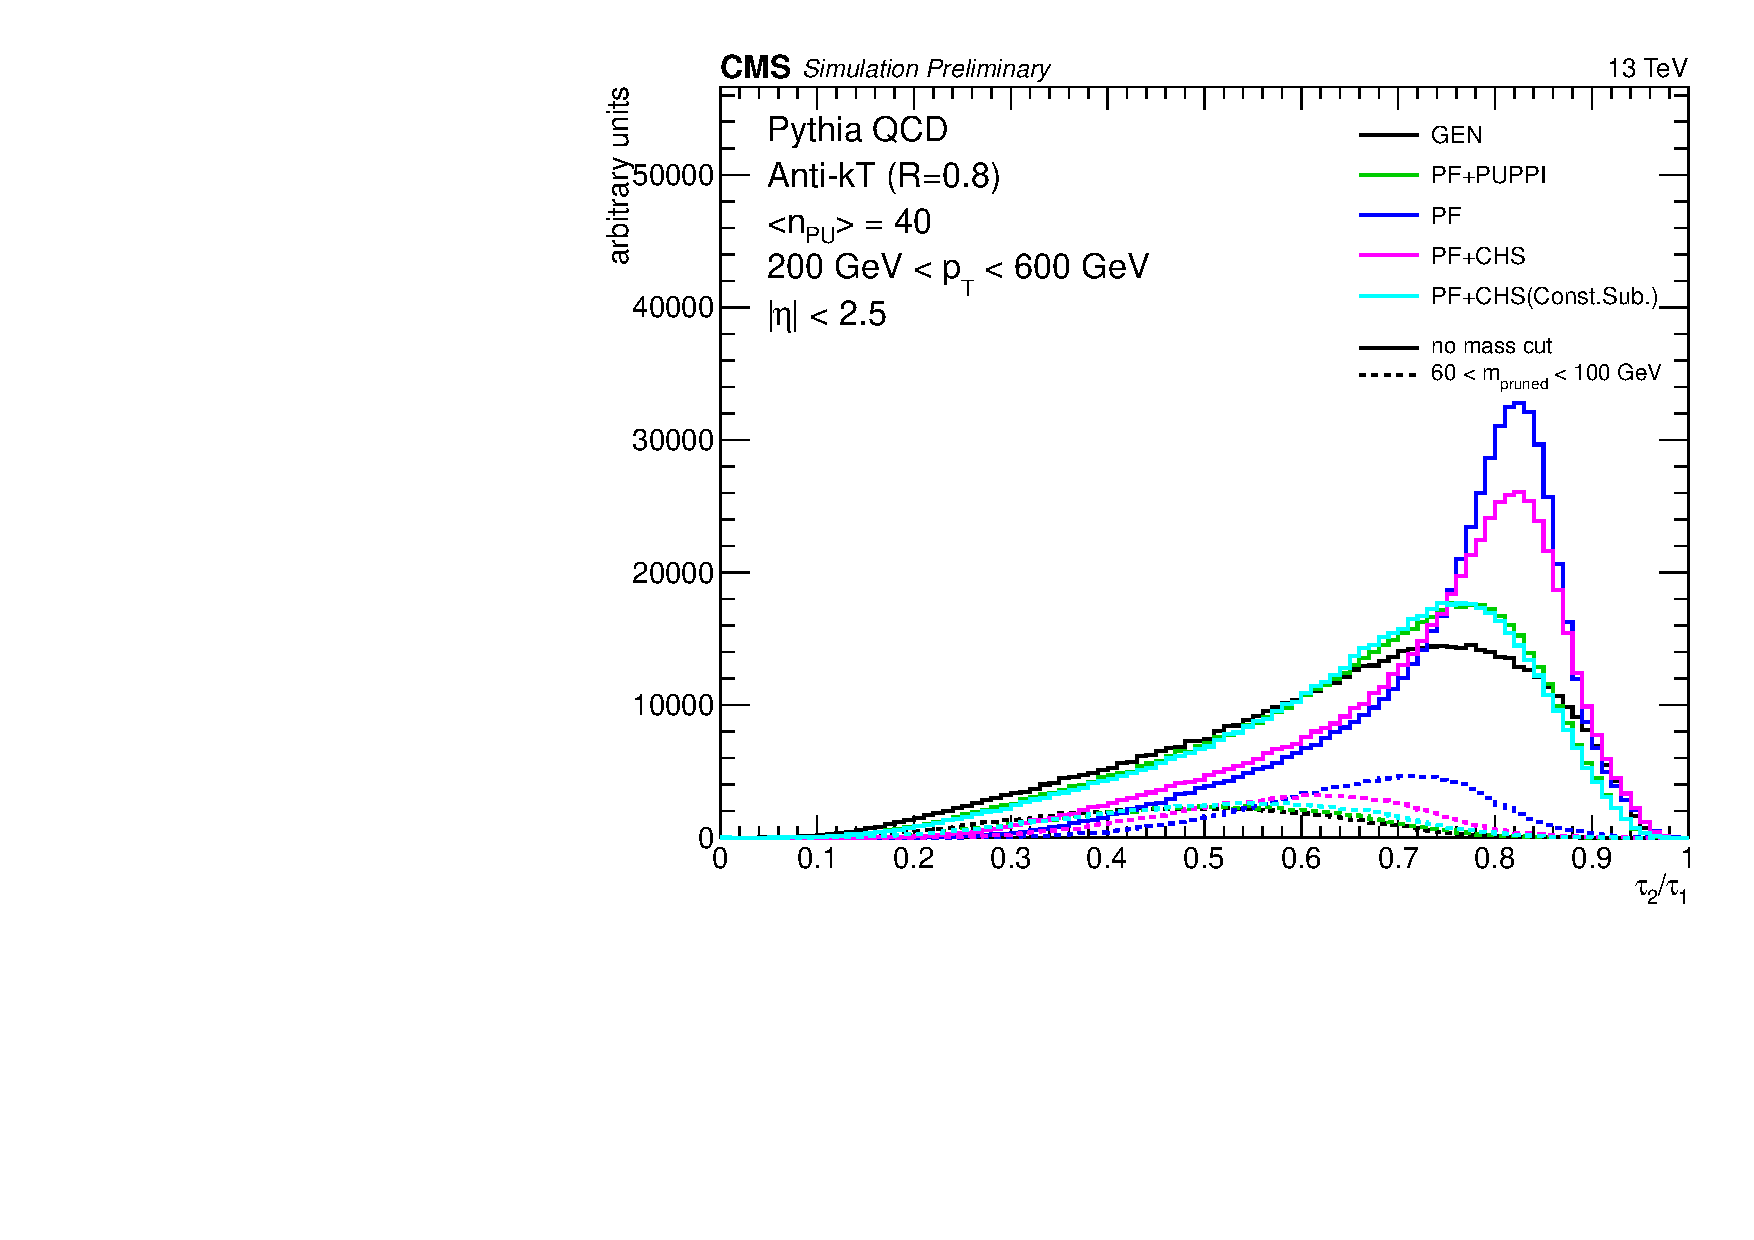
\includegraphics[width=0.490\textwidth]{figures/event_reconstruction/sig_tau21.pdf}
    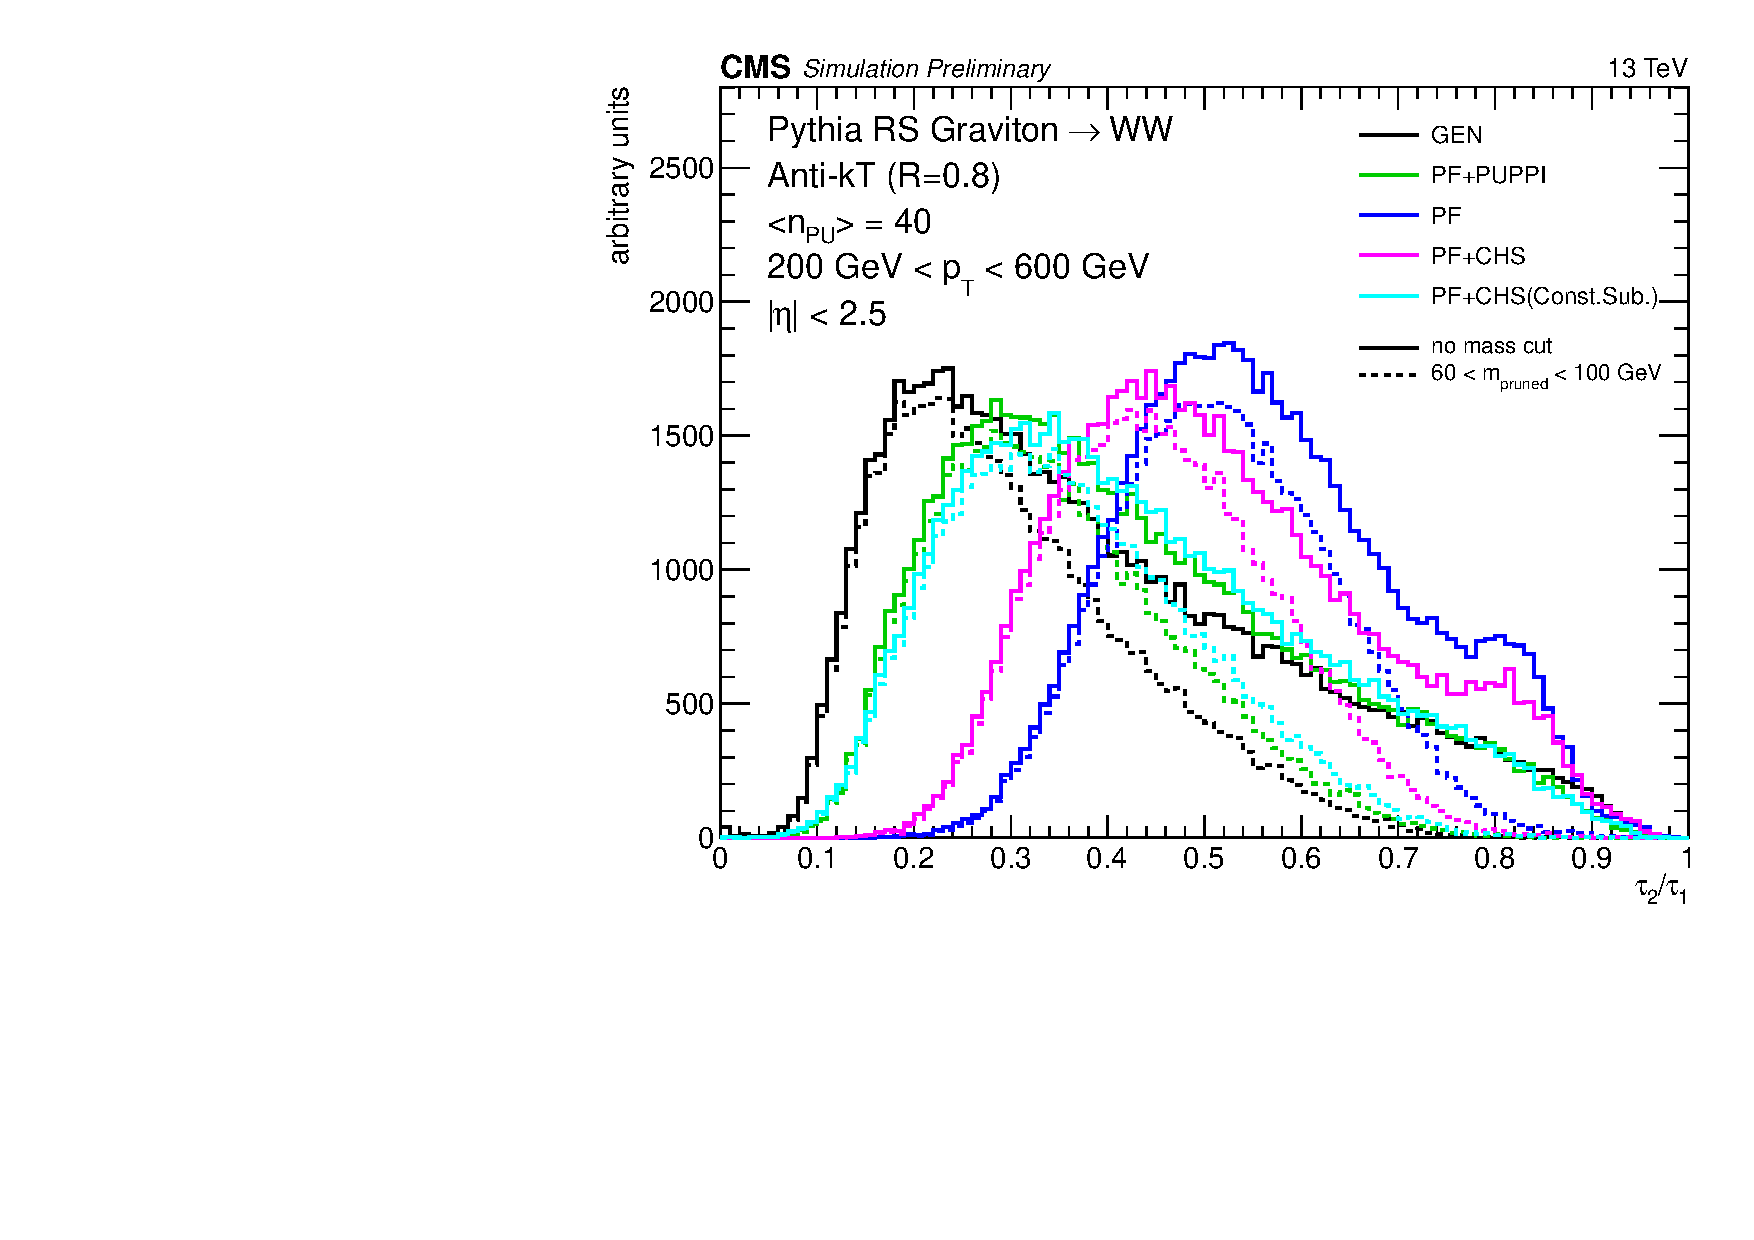
\includegraphics[width=0.490\textwidth]{figures/event_reconstruction/bkg_tau21.pdf}
     \caption{The distribution of the n-subjettiness ratio $\tau_{21}$ for signal jets (left) and background jets (right) with different combinations of pileup subtraction algorithms applied. The solid lines corresponds to the $\tau_{21}$ distribution with no mass cut applied, while the dotted lines are within a mass window of 60-100 \GeV~\cite{CMS-PAS-JME-14-001}.}
     \label{fig:objreco:tau21}
 \end{figure}

\subsection{Vector boson tagging}
In order to discriminate \PW and \PZ bosons from quark/gluon jets a combination of a groomer and shape-tagger (like n-subjettiness) is usually used.
Typical values for tagging W jets is a groomed jet mass between 60 and 100 \GeV and $\tau_{21}<0.5$. The exact combination and value of cuts is analysis dependent, and has been optimized for each search presented in this thesis. The details are thoroughly explained in each section.


\subsubsection{Polarization effects}
\label{sec:objreco:pol}
The vector boson polarization has a significant effect on the W-tagging efficiency. The helicity angle $\theta*$, defined as the angle between the outgoing quark daughters of the W boson in its rest frame relative to its direction of motion~\cite{PhysRevD.86.095031}, is very different for longitudinally polarized vector bosons, \PWL, and transversely polarized vector bosons \PWT ~\cite{Khachatryan:2014vla}. Figure~\ref{fig:objreco:wtwlcostheta} shows the $\cos \theta^*$ distribution for the outgoing quarks from $\PWL \rightarrow q \bar {q}$ (black) and $\PWT \rightarrow q \bar{q}$ (red) decays, and it can be observed that transversely polarized W bosons decay with the quarks emitted closer to the vector boson direction of motion.
\begin{figure}[h] 
    \centering 
    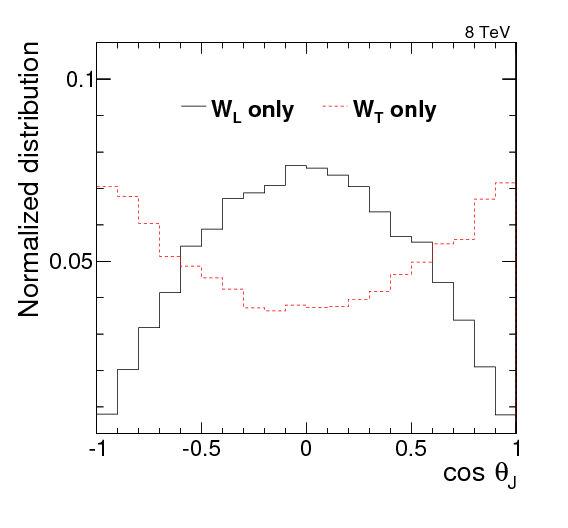
\includegraphics[width=0.5\textwidth]{figures/event_reconstruction/cosThetaJJ_GEN.png}
     \caption{The helicity angle for generated quarks from $\PWL\rightarrow q\bar{q}$ (black) and $\PWT\rightarrow q\bar{q}$ (red) decays~\cite{Khachatryan:2014vla}.}
     \label{fig:objreco:wtwlcostheta}
 \end{figure}
The consequence of this, is that there is a higher asymmetry in the transverse momenta of the two quarks from a \PWT decay. This in turn causes grooming algorithms, designed to remove soft constituents of a jet, tend to reject particles coming from the softer quark, resulting in a lower jet mass and a drop in tagging efficiency. Figure~\ref{fig:objreco:wtwleff} shows the W-jet tagging efficiency versus q/g jet mistagging rate for a selection on the jet pruned mass of $60 \GeV < m_{pruned} < 100 \GeV$, scanning $\tau_{21}$ cuts (here for CA R=0.8 jets).

\begin{figure}[h] 
    \centering 
    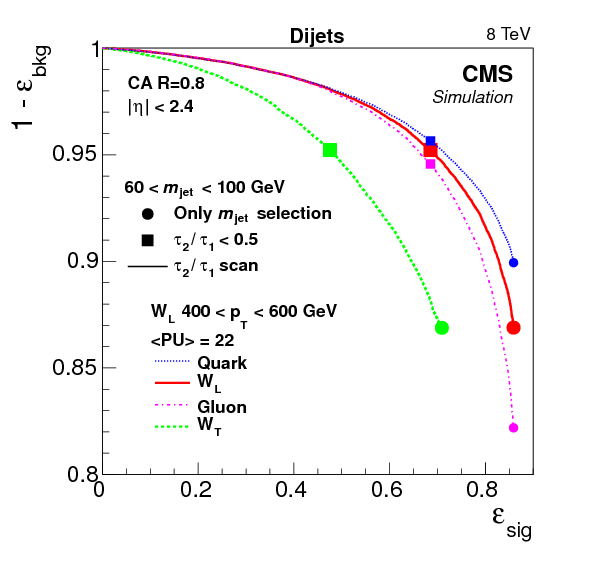
\includegraphics[width=0.5\textwidth]{figures/event_reconstruction/substructure_pas_roc3b.png}
     \caption{The helicity angle for generated quarks from $\PWL\rightarrow q\bar{q}$ (black) and $\PWT\rightarrow q\bar{q}$ (red) decays~\cite{Khachatryan:2014vla}.}
     \label{fig:objreco:wtwleff}
 \end{figure}

The tagging efficiency for transversely polarized W bosons (green) is significantly lower than the tagging efficiency for longitudinally polarized bosons (red). This can be explained by looking at the  $\cos \theta^*$ distribution on reconstructed level, using the C/A subjets, with a cut on the jet pruned mass of $60 \GeV < m_{pruned} < 100 \GeV$, as shown in Figure~\ref{fig:objreco:wtwlcostheta_reco}. When comparing to the distribution at generator level with no groomed mass window applied, Figure~\ref{fig:objreco:wtwlcostheta}, one can see that the \PWT jets with $\cos \theta^ \sim 1$ are completely removed.
\begin{figure}[h] 
    \centering 
    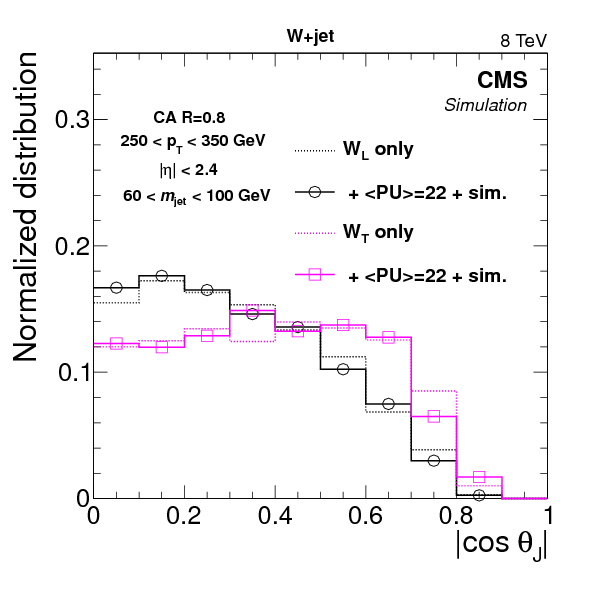
\includegraphics[width=0.5\textwidth]{figures/event_reconstruction/s1vs2-600_sjCosTheta_afterMass.png}
     \caption{The helicity angle for subjets from $\PWL\rightarrow q\bar{q}$ (black) and $\PWT\rightarrow q\bar{q}$ (pink) decays.~\cite{Khachatryan:2014vla}.}
     \label{fig:objreco:wtwlcostheta_reco}
 \end{figure}
 This is due to two effects: the \PT-asymmetry explained above and the fact that the $\Delta R$ distribution between the two quarks is much smaller in the case of \PWL, making them more likely to be fully contained within a jet cone of R=0.8.

\clearpage
\section{Monte Carlo Event Generators}
Monte Carlo event generators offer a realistic estimate of high-energy collisions on an event-by-event basis, allowing us to estimate signal and background processes accurately. Simulated events are usually produced in three steps, beginning with the hard process through hadronization and decay. First, a matrix element generator simulates the hard scattering process and subsequent decays. Secondly, the showering and hadronization of unstable particles is performed and, lastly, the final-state particles are passed through a full detector simulation in order to reproduce a range of experimental effects.\par
General-purpose Monte Carlo (GPMC) generators, like \HERWIG++~\cite{Bahr:2008pv} and \PYTHIA8~\cite{Sjostrand:2014zea}, deal with both perturbative as well as hadronization phenomena, simulating an event all the way up until detector simulation. In \HERWIG++ and \PYTHIA8, the hardest processes are only simulated at the lowest order of perturbative expansion, meaning $2 \rightarrow 2$ or $2 \rightarrow 3$ scatterings. In order to have  tree-level matrix elements with an arbitrary final-state multiplicity, they can be combined with programs used to generate parton-level events at higher accuracy, which are then processed through showering and hadronization with the GPMC generators. One popular program for generating matrix elements is \MADGRAPH~\cite{Aad2015}. This, however, still correspond to a tree-level (leading order) approach. To go to next-to-leading-order (NLO), meaning the inclusion of virtual corrections, two methods exist: \MCATNLO~\cite{Frixione:2002ik,Frixione:2003ei} and \POWHEG~\cite{Frixione:2007vw}. These combine the full next-to-leading-order prediction for inclusive processes with the subsequent parton showers, either by a subtraction method regularizing the real contributions, or by a matrix-element correction of the parton shower branching probability. After hadronization, all final state particles are passed through a full simulation of the CMS detector. This is done with \GEANTfour~\cite{AGOSTINELLI2003250}, which models the interaction and showering of particles with materials, and outputs position-dependent energy deposits.\par
For the work presented in this thesis, simulated samples of the Standard Model background processes are used to optimize the analysis and in some cases provide flexible background templates. QCD multijet production is simulated with four generator configurations: 1. \PYTHIA standalone, 2. the LO mode of \MADGRAPH matched with \PYTHIA, 3. \POWHEG matched with \PYTHIA and 4. \HERWIG{++}~2.7.1 with tune CUETHS1~\cite{Khachatryan:2015pea}. Top-quark pair production is modeled with \POWHEG and showered with \PYTHIA unless otherwise stated. W+jets and Z+jets production are simulated with the leading-order (LO) mode of \MADGRAPH matched with \PYTHIA. Signal samples are generated with standalone \PYTHIA. All samples are processed through a \GEANTfour-based simulation of the CMS detector. To simulate the effect of additional proton-proton collisions within the same or adjacent bunch crossings (pileup), additional inelastic events are generated using \PYTHIA and superimposed on the hard-scattering events. The simulated MC events are finally weighted to reproduce the distribution of the number of pileup interactions observed in data.
